\documentclass{article}

% ---------------------------------------------------------------------------
% PALM @ NeurIPS 2026 — camera-ready version (accepted).
% The workshop template requires BOTH \title{} and \workshoptitle{}.
% "final" de-anonymizes and drops line numbers; drop it to rebuild the submitted version.
% ---------------------------------------------------------------------------
\usepackage[dblblindworkshop, final]{neurips_2026}

\usepackage[utf8]{inputenc}
\usepackage[T1]{fontenc}
\usepackage{hyperref}
\usepackage{url}
\usepackage{booktabs}
\usepackage{multirow}
\usepackage{amsfonts}
\usepackage{amsmath}
\usepackage{amssymb}
\usepackage{nicefrac}
\usepackage{microtype}
\usepackage{xcolor}
\usepackage{graphicx}
\usepackage{subcaption}
\usepackage{tikz}
\usepackage{enumitem}
\usepackage{listings}
\makeatletter
\newcommand{\Needspace}[1]{\par\begingroup\@tempdima=\pagegoal\advance\@tempdima by -\pagetotal
  \ifdim\@tempdima<#1\relax\newpage\fi\endgroup}  % break here if less than #1 is left on the page
\makeatother
\providecommand{\nolinenumbers}{}  % no-op when the final option drops lineno
\lstset{basicstyle=\ttfamily\scriptsize, breaklines=true, breakindent=0pt, columns=fullflexible, keepspaces=true, frame=single, xleftmargin=0pt, framexleftmargin=0pt, aboveskip=4pt, belowskip=4pt}
\setlist[itemize,enumerate]{nosep,leftmargin=*}
\usetikzlibrary{positioning,arrows.meta,calc,shapes.geometric}

% Benchmark name, defined once.
\newcommand{\bench}{DossierBench}

\title{\bench: Scoring a Recommender's Model of You on Calibration, Not Recall}

% The workshop title shown in the footnote.
\workshoptitle{Personalized, Aligned, Long-Term Memory for AI Systems (PALM) @ NeurIPS 2026}

\author{%
  Muhammad Bilal$^{1,2}$ \qquad Jo\~{a}o V. Gra\c{c}a$^{1}$\\
  $^{1}$Soko (\url{https://soko.fyi})\\
  $^{2}$King Abdullah University of Science and Technology (\url{https://kaust.edu.sa})
}

\begin{document}

\maketitle

\begin{abstract}
Recommendation apps increasingly keep a standing preference profile of the user, built from
conversation. The memory systems that build such profiles are evaluated on \emph{recall}, which
rewards committing and cannot see the failure that matters once a profile drives recommendations:
asserting a preference the user never expressed. We introduce \textbf{\bench}, which scores a
profile on \emph{calibration}: does the system commit exactly where the conversation has given it
grounds to? Each synthetic subject is a persona whose dining and going-out preferences are fixed on
a 24-field card and surface gradually over a scripted conversation of many sessions. An
\emph{evidence map} records, for every field at every checkpoint, what the conversation so far has
shown: \textsc{strong}, \textsc{weak}, or \textsc{unevidenced}. A system is served the conversation
one checkpoint at a time and emits the whole card, abstaining where it will not commit. Committing
to an unevidenced field is a fabrication even when the value is right; abstaining there is free.
Fidelity over the timeline is normalized to a skill score with always-abstain at $0$ and an oracle
at $1$. On 50 subjects (612 sessions) and four frontier backbones, two single-pass extractors that
read the conversation directly calibrate well, while a stateful memory layer, evaluated on one
backbone, scores below both at twice the call budget. We release the corpus,
scorer, and reference systems; the benchmark scores the profile alone, before any recommendation is
made.
\end{abstract}

% ===========================================================================
\section{Introduction}
% ===========================================================================

An app that recommends where to eat, drink, or go out is only as good as its model of the user it
serves. Increasingly that model is a standing \emph{preference profile} assembled from
conversation: the user talks to the app over months, and the app maintains what it believes about
their cuisines, budget, noise tolerance, travel radius, and usual company. The recommender conditions
on that profile, so a wrong entry is not an isolated mistake but a standing bias on everything the app
suggests next. The memory systems that build such profiles have largely been optimized for
\emph{recall}: given a fact stated earlier, can the system retrieve it later~\citep{packer2023memgpt,
zhong2024memorybank, chhikara2025mem0}. Recall is necessary, but it is the wrong
top-level target here because it prices only one of the two errors a profile can make. A profile that
forgets a stated allergy recommends a dangerous dish; a profile that \emph{invents} a preference the
user never voiced also misleads the recommender, and a recall metric cannot see it. A system that
commits a plausible value to every field can score well on recall while confidently telling the
recommender that a user who never mentioned wine wants an alcohol-free venue, or that a user likes
Thai food because they once booked a Thai restaurant for someone else.

We argue that the property to measure is \textbf{calibration under evidence}: a profile should commit
to a field exactly when the conversation supports it, and abstain otherwise. We use
\emph{calibration} in this sense, whether the decision to commit matches the evidence, not in the
probabilistic sense of stated confidence matching accuracy. The distinction is
operational, not just epistemic. A field the profile leaves empty is one the recommender can handle
(fall back to a popularity prior, widen the candidate set, or ask), whereas a fabricated field is
one it will silently condition on, with nothing downstream able to tell the two apart. Making that
checkable requires knowing, at each point in a dialogue history, what a careful reader \emph{could}
know. That is the central artifact of this paper: for each subject in the dataset we do not merely store
the ground-truth persona, we derive, from the \emph{evidence schedule} the conversations were written
from (which session reveals which field, and how clearly), an \emph{evidence map} grading every field at every checkpoint as \textsc{strong}, \textsc{weak}, or
\textsc{unevidenced}. The map turns ``the system abstained here'' into a scoreable event: abstaining
on an unevidenced field is correct, abstaining on a strong field is a miss, and committing to an
unevidenced field is a fabrication whether or not the guess is right. We evaluate the profile in isolation: no recommendations are
produced or ranked, and pricing each error by the recommendation it spoils is the next step
(\S\ref{sec:future}).

This paper makes the following contributions:
\begin{itemize}[leftmargin=*]
  \item \textbf{An evidence-conditioned benchmark for preference profiles} (\S\ref{sec:bench}),
  spanning 24 fields (20 preferences and 4 hard constraints) across 8 venue-recommendation groups. Each preference field is scored
  with a type-appropriate metric (set overlap, ordinal distance, or distribution
  divergence), and each hard constraint by whether any item is missed or invented. The harness serves one checkpoint of new dialogue at a time, without re-serving past
  prefixes or revealing the answer key. The 50-subject corpus is \emph{synthetic}: sampled personas
  and evidence schedules, LLM-authored sessions, and an answer key derived from the schedule. The
  dataset and code are released.\footnote{Data: \url{https://huggingface.co/datasets/tangents/dossierbench}; code (scorer, reference systems, prompts): \url{https://github.com/Hey-L-AI/DossierBench}.}
  \item \textbf{A schedule-derived, validated answer key} (\S\ref{sec:map}): the evidence map is
  computed from what the schedule placed; the LLM-reader credit and hand corrections layered on top
  are small, constrained, and recorded, and every map is checked to be monotone.
  \item \textbf{A calibration score with fixed anchors} (\S\ref{sec:scoring}): a fidelity
  trajectory, its area under the curve (AUFC), and a skill normalization pinned so that
  always-abstain $=0$ and the oracle $=1$; negative skill means \emph{worse than emitting nothing}.
  \item \textbf{Reference measurements} (\S\ref{sec:results}): three simple reference systems, two
  single-pass extractors on four frontier backbones (GPT-5.6 Luna, Gemini 3.7 Flash, DeepSeek V4 Pro,
  GLM-5.3 Flash) and one stateful memory layer on GPT-5.6 Luna. Both single-pass extractors clear the
  abstain floor on every backbone; the stateful layer falls below both on its backbone at twice the
  call budget.
  A transcript-grounded failure-mode reading (\S\ref{sec:failures}) traces what each system
  gets wrong and why.
\end{itemize}

% ===========================================================================
\section{Related Work}
\label{sec:related}
% ===========================================================================

\textbf{Conversational recommendation and preference elicitation.} Learning a user's preferences
through dialogue has a long history in recommendation. The system decides what to ask about next. It
may ask for an item to rate \citep{christakopoulou2016towards} or an attribute
\citep{sun2018conversational, lei2020estimation}, and it recommends once it judges it has learned
enough. In that setting an unmentioned attribute is something to ask about. In region-based
elicitation it is an uncertainty set over the user's embedding to shrink \citep{nguyen2024cold}. It
is never a value the system is scored for asserting. An LLM-built profile for recommendation
simulation is scored by the downstream behaviour it produces \citep{wanyan2026task}. That counts a
correct-but-unsupported trait as a success. $\tau$-Rec \citep{narasimhan2026taurec} is the nearest
protocol. Its reveal tags (\texttt{volunteer} / \texttt{on\_ask} / \texttt{hidden}) fix when each
constraint is disclosed. It measures a roughly fourfold drop in success from volunteered to hidden
constraints. But the tags steer only the user
simulator and never enter the reward. The scored artifact is the recommended item, so an agent that
\emph{guesses} a hidden constraint scores exactly as one that learned it from the user's rejections.
Ours is the belief-side instrument to that outcome-side one.

\textbf{Dialogue state tracking.} The nearest experimental instrument to ours is dialogue state
tracking (DST), which tracks typed slots across turns, treating unmentioned slots as absent or
explicit \texttt{none} values \citep{rastogi2020schema, aksu2024granular}. The difference is what
the gold state holds. DST tracks what the user said; we also charge a value that is true of the user
when the transcript has not yet licensed it. DST also cannot represent a hint that narrows a field without
pinning it. Two things follow that have no DST counterpart. One is a three-way evidence band instead of
mentioned-or-not. The other is abstention as a scored positive move instead of the free non-event a
correct \texttt{none} is. We do inherit two metric lessons. Slot accuracy is inflated by the mass of
correctly empty slots \citep{kim2022mismatch}, so our fidelity denominator is fixed to the evidenced
fields. And a per-turn metric re-charges one early error at every later turn
\citep{aksu2024granular}. Our AUFC does this deliberately, since a memory holding a wrong value is
wrong each time it is read.

\textbf{Memory architectures and long-conversation benchmarks.} MemGPT~\citep{packer2023memgpt}
manages a tiered memory with explicit paging. MemoryBank~\citep{zhong2024memorybank} adds forgetting
curves. Mem0 \citep{chhikara2025mem0} extracts salient facts and consolidates them into a bank. These
systems are evaluated by retrieval-style question answering over multi-session
dialogue~\citep{maharana2024locomo, xu2022msc} or long documents. We treat them as \emph{systems
under test} and ask a different question: not ``can you retrieve the fact'' but ``do you know when
you don't know.'' While LoCoMo's adversarial slice credits declining to answer, answerability is treated as a static
per-question label rather than an evolving function of accumulated evidence. Furthermore, on
answerable questions, matching responses receive full credit regardless of whether they were soundly
inferred or guessed. No such benchmark
grades a claim against the evidence state at the time it was made. So none separates a correct
abstention from a lucky guess, and none prices a fabrication that happens to be right.

\textbf{Evidence-conditioned scoring of inferred profiles.} The failure we target is asserting a
preference the conversation does not support. It has only recently been measured directly.
MirageBench \citep{sun2026miragebench} comes closest. It scores inferred user-profile claims on
\emph{evidential support rather than truth}, and it labels a claim that goes beyond the revealed
evidence as over-inference ``regardless of whether \dots\ [the profile] agrees with it.'' Its authors
call for stored user information to be tagged with its epistemic status, which is the three-way
banding we compute. It differs from our setting in exactly the ways that motivate ours. Its evidence
is a fixed handful of revealed facts rather than a growing prefix. Each claim is judged once rather
than re-scored as the transcript accumulates. And abstention is invisible: its over-inference rate is
a ratio over \emph{emitted} claims, and no metric credits coverage. GISTBench
\citep{fostiropoulos2026gistbench} is the nearest in stance: it verifies each inferred interest
against the engagement signals cited for it rather than against a label, but has no abstention
channel and scores a single snapshot per user. The neighbouring benchmarks fall on one side or the
other of the same line. Some \emph{reward} the unevidenced generalization we penalize. Some drop
unevidenced fields from the question set, so honest abstention cannot be expressed. And some score an
explicit \texttt{unknown} below a wrong guess. Appendix~\ref{app:relwork} works through each.
Our stance descends from fact verification against retrieved evidence \citep{thorne2018fever} and
from calibration work asking whether a model knows what it knows~\citep{kadavath2022know}.

% ===========================================================================
\section{The Benchmark}
\label{sec:bench}
% ===========================================================================

\textbf{Domain and persona.} The domain is venue and event recommendation: restaurants, bars,
caf\'es, and things to go to. Each subject is defined by a \emph{persona card} of 24 fields in 8
domain groups, from hard constraints (dietary restrictions, allergies, accessibility, alcohol-free
requirements) to taste, ambiance, logistics, and events (Appendix~\ref{app:fields}). The groups match how a recommender uses them:
hard constraints are filters (a venue is removed, not moved down the list); taste, ambiance,
and quality signals are ranking features; and the three distribution fields (price band, party
size, visit time) are what a booking step must fill in to hold a table at all. Each preference field is scored
by an agreement score $a_f\in[0,1]$ suited to its type: set overlap for the set-valued fields,
distance along the scale for the ordinal fields, and a
divergence for the three distributions over bins. The fidelity score (\S\ref{sec:scoring})
averages $a_f$ over the evidenced preference fields; the four hard constraints are checked
separately, item by item.

\textbf{Conversations.} A subject's history is a sequence of dated sessions between the user and a
recommendation-and-booking assistant: asking for somewhere to eat, reacting to suggestions,
booking a table, reporting back afterwards. Sessions are written so that each field becomes
knowable only where the schedule places evidence for it, and \emph{fenced} so that no field leaks
into a session that was never meant to reveal it; some sessions are distractors that reveal nothing
new. Subjects run from 3 to 30 sessions (median 8), each about eight messages and 230 words.
Section~\ref{sec:corpus} describes the pipeline that produces them.

\textbf{Serving protocol.} Conversations are evaluated chronologically across discrete
checkpoints, written $c_0, c_1, \ldots$ and counted from 0; in this corpus each checkpoint adds one session. At checkpoint $t$ the system is
given \emph{only} the sessions new since $t-1$ and must return the entire persona card, using an
explicit \texttt{unknown} for any field it will not commit to; on a preference list field an empty
list is a commitment (``none''), not an abstention. Two rules are built into the
harness rather than left to the system:
\begin{enumerate}
  \item \emph{Earlier sessions are never re-served.} Carrying earlier text forward is the system's own
  choice. Replaying the full transcript is a different, easier benchmark.
  \item \emph{The answer key is never served.} The answer key is the gold card plus the evidence
  map (\S\ref{sec:map}). The system sees transcripts and dates only; the schedule and the answer
  key stay held out.
\end{enumerate}
A system under test is encapsulated behind a minimal stateful interface implementing
\texttt{reset} and \texttt{observe(new\_sessions) $\rightarrow$ card}. Any memory design can
implement it.

% ===========================================================================
\section{Corpus Construction}
\label{sec:corpus}
% ===========================================================================

Every subject is built by the five-stage pipeline of Figure~\ref{fig:pipeline}. The plan (Stages
1--3: card, timeline, and evidence schedule) is fixed by a seed, the session text written from it
in Stage~4 is released as a frozen copy with checksums, and the answer key of Stage~5 starts from
the plan (\S\ref{sec:map}).

\begin{figure}[t]
  \centering
  \footnotesize
  \resizebox{\linewidth}{!}{%
  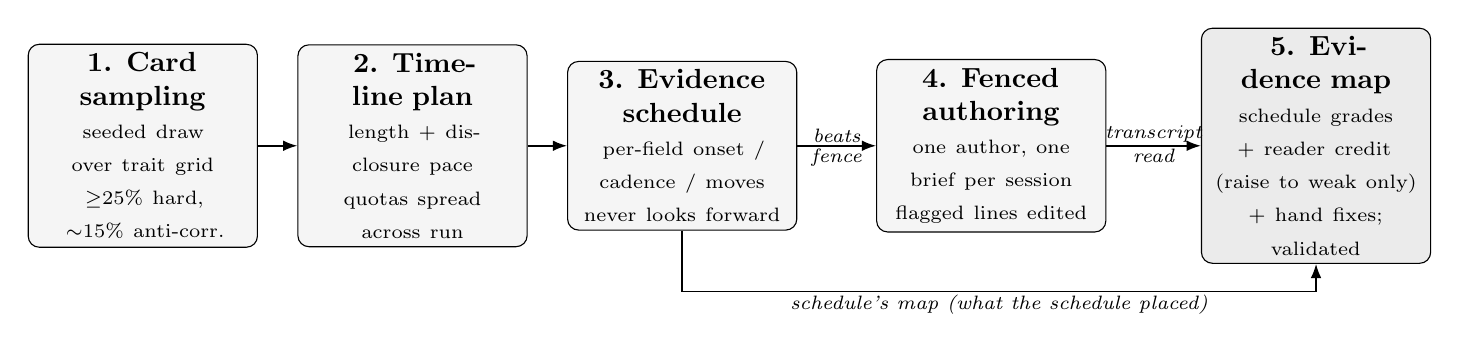
\begin{tikzpicture}[
    node distance=5mm and 5mm,
    stage/.style={draw, rounded corners, align=center, inner sep=3pt,
                  minimum height=13mm, text width=27mm, fill=black!4},
    lbl/.style={font=\scriptsize\itshape, align=center, inner sep=1pt},
    arr/.style={-{Latex[length=1.8mm]}, semithick},
  ]
    \node[stage] (card) {\textbf{1. Card sampling}\\{\scriptsize seeded draw over trait grid}\\{\scriptsize $\ge$25\% hard, $\sim$15\% anti-corr.}};
    \node[stage, right=of card] (plan) {\textbf{2. Timeline plan}\\{\scriptsize length + disclosure pace}\\{\scriptsize quotas spread across run}};
    \node[stage, right=of plan] (sched) {\textbf{3. Evidence schedule}\\{\scriptsize per-field onset / cadence / moves}\\{\scriptsize never looks forward}};
    \node[stage, right=10mm of sched] (auth) {\textbf{4. Fenced authoring}\\{\scriptsize one author, one brief per session}\\{\scriptsize flagged lines edited}};
    \node[stage, right=12mm of auth, fill=black!8] (map) {\textbf{5. Evidence map}\\{\scriptsize schedule grades + reader credit}\\{\scriptsize (raise to weak only)}\\{\scriptsize + hand fixes; validated}};

    \draw[arr] (card) -- (plan);
    \draw[arr] (plan) -- (sched);
    \draw[arr] (sched) -- node[above,lbl]{beats} node[below,lbl]{fence} (auth);
    \draw[arr] (auth) -- node[above,lbl]{transcript} node[below,lbl]{read} (map);
    \draw[arr] (sched.south) |- ($(map.south)+(0,-3.5mm)$) -- (map.south);
    \node[below,lbl] at ($(sched.south |- map.south)!0.5!(map.south)+(0,-3.5mm)$) {schedule's map (what the schedule placed)};
  \end{tikzpicture}%
  }
  \caption{The corpus-construction pipeline. Stages 1--4 produce a subject's gold card and dated
  conversation; Stage~5 builds the evidence map from the grades the schedule placed, plus a small
  reader-credit layer and a few recorded hand corrections (\S\ref{sec:map}). The transcript is served to the system and the held-out
  map to the scorer.}
  \label{fig:pipeline}
\end{figure}

\textbf{Stage 1: Card sampling.} A persona card is \emph{drawn} at random, from a seed, over a
declared grid of trait values, not asked of a model. Drawing rather than prompting lets us \emph{build
in} coverage instead of checking it afterwards. The draw gives a spread across the grid that can be
audited, and meets two quotas. At least 25\% of subjects are hard cases of one of four kinds: a
stated preference that the scheduled behaviour contradicts, a hard constraint guaranteed to come up
only once, with the session text checked so it is never raised again, a two-peaked price or visit-time distribution, or a few strong traits set against
mid-scale values everywhere else. About 15\% are anti-correlated cases: they intentionally violate one of the declared correlation
clusters (C1 exploration, C2 spend, C3 sociality, C4 deliberateness; details in Appendix~\ref{app:fields}) by a measurable
margin, so a system cannot score by assuming clusters always hold together. No model is involved in
this stage: a fixed rule check rejects a card whose values contradict each other or that gives the
author nothing distinctive to voice, and never rejects one for being atypical.

\textbf{Stage 2: Timeline planning.} Each subject is assigned a conversation length and a pace at
which it reveals itself. There are no difficulty tiers: evidence is thin early in every timeline and
dense late, so a system passes through every density of evidence within a single subject.

\textbf{Stage 3: Evidence schedule.} This stage decides \emph{where} each field becomes knowable.
Every field has its own plan with three parts: an onset (the session it first surfaces in, drawn from
an exponential distribution whose rate is the subject's pace), how often it recurs, and a sequence of
moves that go from narrowing (a reaction, an anecdote) to pinning the value down. The one rule the
scheduler enforces is that \textbf{it never looks forward}: the \emph{beats} of session $i$ (the pieces of evidence planned for it) depend only on the
seed, the subject id, and the sessions before $i$, never on the total length. So a timeline can be
extended without changing what came before: raising a subject from 8 to 25 sessions leaves the first
8 unchanged. It is also where the \textsc{unevidenced} band comes from: a field with a late onset
simply never surfaces in a short timeline.

\textbf{Stage 4: Fenced authoring.} One author model (Claude Opus 5 here) turns the schedule into
dated sessions. Each session is written from its own brief (its beats, its date, and the date of the
previous conversation), never from the text of earlier sessions, so what a session is meant to reveal is set by
the schedule alone. The corpus contains
no scripted changes of mind, so a value once evidenced stays true and a grade never has to be walked
back. The author is shown the whole person but \emph{fenced}: it may reveal only the beats the
schedule placed in that session. The fence keeps the unevidenced band honest. Without it, an
in-character aside (``I'll have the extra chilli'') would leak a field (spice tolerance) the key
records as unknown. After authoring, two LLM \emph{fence checkers} checked every session, and an editor model (Claude Opus 5) rewrote only the
messages they flagged as breaking the fence or the brief, leaving the rest of the session
untouched; a small number of sessions were fixed by hand. 293 of the 612 released sessions
carry at least one such edit.

\textbf{Stage 5: The evidence map.} The grades the schedule placed are the starting evidence map.
Two LLM \emph{evidence readers} on different models (Claude Opus 5 and Sonnet 5 here) then read every session for
evidence the schedule did not place; \S\ref{sec:map} gives the rules for what they may change.

% ===========================================================================
\section{The Evidence Map}
\label{sec:map}
% ===========================================================================

The evidence map is what makes calibration checkable. Each cell grades one field at one checkpoint
by what the sessions served so far show: \textsc{strong} if they pin the value, \textsc{weak} if
they bear on it without pinning it, and \textsc{unevidenced} if nothing in them bears on it yet.
The map's core, the \emph{schedule's map}, is computed from the schedule. Any evidence makes a field
at least \textsc{weak}; it becomes \textsc{strong} once enough pinning evidence has accrued. One
direct request, or a rejection that says what was wrong, pins an ordinal field or a hard
constraint; a set field needs two, and a distribution five occasions. A reaction to a visit or a
passing anecdote narrows a field but never pins it. Evidence comes from three sources:
\begin{itemize}
  \item a \textbf{beat}, the field's own evidence in the subject's voice, which can raise a grade and
  is weighted by how strong it is;
  \item an \textbf{occasion}, the party size, time, and price band a session must state simply to
  book a table, which counts as incidental evidence for the matching distribution field
  whether or not a beat asked for it;
  \item a \textbf{trait implied by an occasion}, credited only up to \textsc{weak} and only where
  the field has no evidence of its own (e.g.\ a party of one is weak evidence for
  solo-dining comfort). The credit says only that the field has been narrowed, not which way,
  since an anti-correlated subject can break the usual pairing.
\end{itemize}
The schedule's map has two properties by construction: it is \textbf{prefix-stable} (appending
future sessions cannot alter past grades, because the scheduler never looks forward) and
\textbf{monotone} (it only adds evidence, so a field's grade never decreases across checkpoints).
Figure~\ref{fig:map} (Appendix~\ref{app:fields}) shows the map for one 16-session
subject: bands only ever darken left to right, six fields the schedule never touches stay
unevidenced for the whole timeline, and each cell fixes whether committing or abstaining is the
right move at that checkpoint. Appendix~\ref{app:example} traces one session through these rules.

\textbf{What counts as evidence.} The key, the reference prompts, and every LLM reader apply one
written policy (stated in full in the prompts of Appendix~\ref{app:prompts}). Only what the user
says, orders, chooses, or rejects counts; what the assistant offers or describes does not, even
about a place the user then books. Booking a venue is not liking its cuisine, and a companion's
needs are not the user's. Where a claim and the user's behaviour disagree, the behaviour counts. A
value is credited under the word the user used, not a neighbouring one (sushi is not
\texttt{japanese}).

\textbf{Reader credit and hand corrections.} Two small, recorded layers sit on top of the
schedule's map. A page can carry more than its beats (booking a table for tonight states a planning
horizon), so a cell the schedule left \textsc{unevidenced} is raised to \textsc{weak} where both
evidence readers find the field readable on the page and the gold card holds a value for it; where
only one finds it, or either flags a leak or a contradiction, a human rules on the full
transcript. An evidence reader can never lower a grade, raise one to \textsc{strong}, or introduce a value the
card does not hold. Separately, cells found to be keyed wrongly were corrected by hand against
the transcript, each as a recorded edit to one field from a stated checkpoint on, and 86
gold-card values in 45 subjects were corrected by hand the same way, most of them by removing a list
item the transcript never voiced. Every
\textsc{strong} cell is still the schedule's own. Of the 14,688 field-checkpoint cells, 4,464 are
\textsc{strong}, 5,244 \textsc{weak}, and 4,980 \textsc{unevidenced}; 225 (1.5\%) differ from the
schedule's grade (breakdown in Appendix~\ref{app:fields}). Every score in this paper is on this
final key.

\textbf{Validation.} A finished map must pass a consistency check before it can serve as an answer
key: a field graded knowable at checkpoint $t$ must remain at least that knowable at $t+1$, so a
system is never asked to know a fact and then to have forgotten it. A reader-credit raise comes only from a
session already served, so prefix-stability is kept. All 50 released subjects pass.

% ===========================================================================
\section{Scoring: Fidelity, AUFC, and Skill}
\label{sec:scoring}
% ===========================================================================

Fidelity covers the 20 preference fields. The four hard-constraint fields never enter it: they are
scored separately by the hard-constraint failure rate (below), so a constraint error is not charged
twice. Let $S(t)$, $W(t)$, $U(t)$ be the sets of preference fields graded
strong, weak, and unevidenced at checkpoint $t$, with one exclusion: a distribution field graded
weak is left out of all three, because a histogram's shape cannot be read from the handful of
occasions behind a weak grade, so it is neither scored nor counted as a fabrication. For a field
$f$ the system under test either commits a value, scored by its metric $a_f\in[0,1]$ against the
gold card in force at checkpoint $t$, or emits \texttt{unknown}. The gold at $t$ is not always the
final card: for the four cuisine and event-type lists it holds only the items the conversation has
shown so far, and for five ordinal fields it is the highest level the user's turns support so far
(fields listed in Appendix~\ref{app:fields}); every other field is scored against the final card.
The per-band rule is:

\begin{center}
\begin{tabular}{@{}lll@{}}
  \toprule
  Band & Commit a value & Emit \texttt{unknown} \\
  \midrule
  $S(t)$ strong & scored $a_f$ & scored $0$ (a miss) \\
  $W(t)$ weak   & scored $a_f$ & scored \textsc{weak-credit} $=\nicefrac{5}{6}$ \\
  $U(t)$ unevidenced & $-\lambda$ penalty (fabrication) & scored $0$ (correct abstention) \\
  \bottomrule
\end{tabular}
\end{center}

The constant $\textsc{weak-credit} = \nicefrac{5}{6}$ is set so that a system reading a weak field
exactly as far as the evidence goes gains nothing by either committing or abstaining. It is derived
for four-level ordinal fields, 13 of the 20 scored: when the evidence narrows such a field to two
adjacent levels, a 50/50 guess between them scores $\frac{1}{2}(1 + \frac{2}{3}) = \nicefrac{5}{6}$
on average, so committing pays only if the system has signal beyond the narrowing. The set fields
take the same constant by convention; Appendix~\ref{app:resultstable} varies it by $\pm 0.08$.
Let $\operatorname{score}(f,t)$ denote the per-field score for evidenced fields $f \in S(t)\cup W(t)$ in the table, and let
$C_U(t)=\{f\in U(t): f\text{ is committed}\}$ be the set of fabrications. The fabrication penalty
is
\[
  \operatorname{Pen}(t)=\lambda\,|C_U(t)|, \qquad \lambda=1.
\]
With $\lambda=1$ a fabrication costs exactly what a miss on a strong field costs, so one fabrication
cancels one correct commit. The value is a stated position, not a fitted one
(\S\ref{sec:limits}); every gap reported in \S\ref{sec:results} is rechecked under
$\lambda\in\{0.5,1,2\}$, crossed with the other two scorer settings, and those reported as real hold
under all 27 (Appendix~\ref{app:resultstable}).
The fidelity at checkpoint $t$ is therefore
\[
  F(t)=\frac{\displaystyle\sum_{f\in S(t)\cup W(t)}\operatorname{score}(f,t)
  -\operatorname{Pen}(t)}{|S(t)|+|W(t)|}.
\]
Its denominator is fixed by the map rather than by the system's decisions. Let
$T_e=\{t: |S(t)|+|W(t)|\ge 7\}$ be the eligible checkpoints (5 and 10 are checked in
Appendix~\ref{app:resultstable}), so the headline number is not dominated by thin early
checkpoints. The \textbf{Area Under the Fidelity Curve (AUFC)} is
\[
  \mathrm{AUFC}=\frac{1}{|T_e|}\sum_{t\in T_e}\min\bigl(1,\max(0,F(t))\bigr).
\]
Skill is normalized per checkpoint. Because abstaining on a
weak field earns credit, a card that abstains everywhere scores not $0$ but
$F_0(t)=\textsc{weak-credit}\cdot|W(t)|/(|S(t)|+|W(t)|)$, and skill rescales the unclipped $F(t)$
against that floor:
\[
  \operatorname{skill}(t)=\frac{F(t)-F_0(t)}{1-F_0(t)}.
\]
A system that always emits \texttt{unknown} therefore scores exactly $0$ at every checkpoint, and an
\emph{oracle} that commits the gold value wherever the map grades a field evidenced scores $1$, so negative skill has a concrete meaning: \emph{worse
than emitting nothing}. A subject's \textbf{skill} is the mean of $\operatorname{skill}(t)$ over its
eligible checkpoints, and the reported skill is the mean over subjects with at least one eligible
checkpoint. Skill is therefore not AUFC rescaled after averaging, and, being unclipped, it can fall
well below $-1$. We report skill; the paired significance tests compare per-subject AUFC
(Appendix~\ref{app:resultstable}).

\textbf{Hard constraints.} The \textbf{hard-constraint failure rate} is the share of subjects with
at least one checkpoint on which the emitted card misses or invents a member of one of the four
hard-constraint fields. A missed member counts only once the field is evidenced; an invented one
counts at any checkpoint. An \texttt{unknown} on an evidenced constraint field with a non-empty gold
value is a miss: a filter failure in its own right, reported beside skill and never averaged into
fidelity.

\textbf{Zero-cost baselines as checks.} Four baselines that need no model calls check the key and
harness: the oracle and \texttt{abstain} land exactly on their anchors, and the population prior and
random land near skill $-4$, fabricating on every unevidenced field (Appendix~\ref{app:gate}).

% ===========================================================================
\section{Experiments}
\label{sec:results}
% ===========================================================================

\textbf{What these numbers are for.} The measurements below are reference points, not a leaderboard:
they show that the score separates real systems, that its anchors sit where the construction says
they do, and that the failures it penalizes are ones systems like those deployed today actually make
(caveats in \S\ref{sec:limits}). Each \emph{(system, backbone)} cell is a single run; the paired confidence
intervals (Appendix~\ref{app:resultstable}) resample \emph{subjects} within it, so they cover variation across subjects, not
run-to-run randomness.

\textbf{Systems under test.} We test three deliberately simple reference systems that differ in
call budget and carried state (diagrams in Appendix~\ref{app:suts}).
\texttt{prompted} spends one call per checkpoint: it is shown the card it last emitted plus the new
sessions and emits the card again, so the card is all the model carries forward. \texttt{notebook} is the
same loop with a free-text scratchpad it writes to itself and is shown back, testing whether
free-form notes buy anything over the card alone. \texttt{memory} spends two calls: an
\emph{extract} call reads only the new sessions and writes candidate memories, and an
\emph{integrate} call, which never sees the conversation, merges them into a persistent bank and
rebuilds the card from it. All three carry state across checkpoints. We call \texttt{prompted} and
\texttt{notebook} \emph{single-pass} because one call reads the new sessions and writes the card; we
call \texttt{memory} \emph{stateful} because its card is rebuilt from a separate bank by a call that
never sees the conversation. All three also carry a running count of occasions for the three
distribution fields, held by code rather than by the model (Appendix~\ref{app:suts}). Because earlier
sessions are never re-served (\S\ref{sec:bench}), what each system carries beyond those counts is
exactly what it chooses to hold. All three run on fixed system prompts that state the evidence
policy of \S\ref{sec:map}; the field menu comes in the user turn of every
call except \texttt{memory}'s extract call (Appendix~\ref{app:prompts}).

The two single-pass systems are run on four frontier backbones: GPT-5.6 Luna, Gemini 3.7 Flash, DeepSeek
V4 Pro, and GLM-5.3 Flash; \texttt{memory} is run on GPT-5.6 Luna only (routes, providers, and reasoning settings in
Appendix~\ref{app:suts}). A results row is a
\emph{(system, backbone)} pair, because the same design behaves differently on different
backbones.

\textbf{Reference measurements.} Figure~\ref{fig:results} reports skill by system and backbone over
all 50 subjects (47 enter the mean; three never reach the seven evidenced fields an eligible checkpoint needs,
\S\ref{sec:scoring});
Appendix~\ref{app:resultstable} gives the same numbers as a table. \textbf{The single-pass extractors are well calibrated}: every bar clears the abstain
floor by a wide margin, from a little under half the distance to the oracle (GLM-5.3 Flash) to about four
fifths (Gemini 3.7 Flash). \textbf{The
backbone matters more than the system}: changing backbone moves skill by up to $0.36$, changing
between the two single-pass systems on the same backbone by at most $0.06$. \textbf{A free-text scratchpad provides no consistent benefit}: the \texttt{prompted}/\texttt{notebook}
order flips by backbone, and only the Gemini 3.7 Flash gap survives a paired bootstrap over subjects on AUFC
and holds under every scorer setting we tried (Appendix~\ref{app:resultstable}). A free-text
scratchpad therefore neither reliably helps nor hurts a single-pass system.

For the stateful system we have a single cell, reported in text rather than in
Figure~\ref{fig:results}: \texttt{memory} on GPT-5.6 Luna scores $+0.493$, against
$+0.669$/$+0.700$ for the single-pass systems on the same backbone, with a hard-constraint failure
rate of $0.30$ against $0.08$--$0.14$ (\texttt{abstain}: $0.56$). The gap to both single-pass systems is significant and holds
under every scorer setting (Appendix~\ref{app:resultstable}). It still clears the abstain floor,
so on this backbone the memory layer costs skill but stays above silence; \S\ref{sec:failures}
says what it loses instead.

\begin{figure}[t]
  \centering
  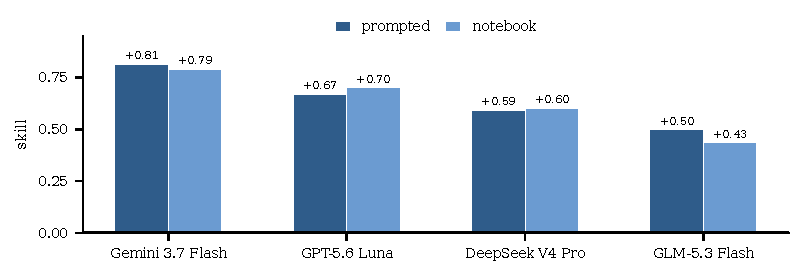
\includegraphics[width=0.9\linewidth]{fig_results.pdf}
  \caption{Skill (\texttt{abstain} $=0$, \texttt{oracle} $=1$) of the two single-pass systems by
  backbone; 50 subjects. The stateful system (\texttt{memory}) is reported in the text.}
  \label{fig:results}
\end{figure}

\subsection{What the systems get wrong}
\label{sec:failures}

The score says \emph{how much} a system fabricates; the released transcripts let us ask \emph{what
kind} of mistake each one is. We grouped every cell the scorer charged (a commit scoring below $0.5$, a fabrication, or a missed
or invented constraint item; an \texttt{unknown} on a strong preference field is not included) on
the nine runs of
\S\ref{sec:results} (each on all 50 subjects) into 807 \emph{episodes}; a field wrong with the same
value across consecutive checkpoints counts once. LLM \emph{failure readers}, blind to which system produced an
episode, read each distinct case (episodes sharing subject, field, values, and first checkpoint are
read once) against the full served transcript under the answer key's written evidence policy, and
every case not judged a genuine error was read a second time, independently
(Appendix~\ref{app:failures}). The \emph{confirmed mistakes} (episodes judged genuine system errors
rather than artifacts of the key) show five patterns.

\textbf{Committing too early is the main failure, and it does not pay.} Between 49\% (DeepSeek V4
Pro) and 74\% (GLM-5.3 Flash) of each backbone's single-pass confirmed mistakes are commits on a field
the transcript has not yet evidenced, 45\% of them at the very first checkpoint. The guess is in the
final gold card in at most 17\% of episodes, so even checked against the hidden card, the guess is
mostly wrong.

\textbf{The guess is the middle of the scale.} On the ordinal fields, 266 of 323 errors
are commits on an unevidenced field, and the level committed is the middle of the scale
whatever the persona (level codes in Appendix~\ref{app:fields}): \texttt{notices\_value} for
\emph{deal-seeking}, \texttt{fine\_with\_lively} for \emph{noise}, one of the two middle levels for
\emph{design}. One mechanism does lean one way: every backbone reads \emph{formality ceiling} off
the \emph{current} occasion, so one counter-service request at $c_0$ becomes the ceiling.

\textbf{Which cells fail varies by backbone; what triggers a failure is shared.} Of the (subject,
field) cells that any single-pass backbone fails on \texttt{prompted}, 64\% fail under one backbone
only and 5\% under all four. What is shared is the \emph{trigger}: a per-head budget cap becomes a
deal-seeking level; a format chosen or praised becomes an event type (\texttt{market}, the
most-invented event type, on all nine runs); a soft preference becomes a hard constraint (``a proper
table rather than perching'' $\to$ \texttt{seating\_required}, 74 episodes). Nearly every invented
list element we traced has a line in the text behind it before the commit; the failure is in
deciding what counts as evidence, not in remembering. Some of these lines are judgment calls a human
could draw differently (a proper table rather than perching read as a seating need); the key settles
each by one written policy, which the prompts state.

\textbf{A single-pass system can also throw away what it holds.} Told to record only what the person
says, some backbones apply that to the \emph{carried card} as well as the new batch. At such a
\emph{wipe}, five or more held fields are rewritten to \texttt{unknown} at once and the card is
rebuilt from the current sessions, though nothing in them contradicts what was held.
\texttt{prompted} wipes 16 times on DeepSeek V4 Pro and never on the other three backbones;
\texttt{notebook} wipes 3--6 times on every backbone. Hard constraints suffer most because most are mentioned only
once: 33 of DeepSeek V4 Pro \texttt{prompted}'s 42 constraint drops sit inside a wipe. A prompt
for such a system should say that what it holds stands unless contradicted.

\textbf{A memory layer changes the kind of failure, not only the amount.} The one stateful run
(\texttt{memory} on GPT-5.6 Luna) has more than $3\times$ the confirmed mistakes of the single-pass
systems on the same backbone (3.14 per subject against 0.84--0.90), and its mix shifts toward loss:
36\% of its episodes are losses (a held constraint gone in a session that does not mention it, a
distribution frozen on one occasion, a repeatedly evidenced value overwritten by one contrary line),
against 11--14\% for the single-pass systems on that backbone. Single-pass errors persist (median
length 3--5 checkpoints; the wrong value rides forward on the carried card) while stateful errors flicker
(median length 1; 20\% of its wrong cells go wrong, right, wrong again, against 0--3\% single-pass on
the same backbone). The raw outputs of the two calls point to the protocol rather than the backbone, though one
backbone cannot confirm it:
the card is re-read from the bank at every checkpoint with no
previous card shown, so a vague memory (``enough room to turn'') is mapped onto the schema afresh
each time; contradictions are \emph{added} to the bank rather than superseding what they contradict;
and 42\% of the distribution data points match no bin and are dropped, starving those fields of
data. That last one is a gap in our reference implementation, not in memory layers as such: the
extract call is never shown the bin names (Appendix~\ref{app:prompts}). The same unstable re-read, not a single early drop, is behind its
higher hard-constraint failure rate (\S\ref{sec:results}).

% ===========================================================================
\section{Limitations and Future Work}
\label{sec:limits}
% ===========================================================================

\textbf{We score the profile, not the recommendations.} \bench{} measures the fidelity of a
preference profile against what the conversation evidenced; it produces no ranked list of venues and
evaluates no recommendation. The assumption that a better-calibrated profile yields better
recommendations, and in particular that a fabricated field costs more downstream than an abstention,
motivates the score but is not measured here. The fabrication penalty
should be read as a stated position on what a profile owes a recommender, not as a measured
estimate of the harm done downstream.

\textbf{Coverage of the measurements.} The single-pass systems are measured on all 50 subjects and
all four backbones; the stateful layer is measured on one backbone (\texttt{memory} on GPT-5.6
Luna), and each cell is a single run. The
failure-mode reading of \S\ref{sec:failures} relies on LLM failure readers (Appendix~\ref{app:failures}).
They found the answer key itself wrong on six fields: four are corrected in the released key, and two remain (2 of the 807 episodes, 0.2\%; Appendix~\ref{app:failures}). They also doubted 55 more gold questions (single-reader calls, kept as keyed;
Appendix~\ref{app:failures}); a human review of the key is next. One credit rule also reads the
hidden card: an outing counts as evidence for the formality ceiling only when it is at the
subject's ceiling (about 240 cells); a rule that reads the page alone is planned for the next
release. All four backbones are general-purpose frontier
models and the reference systems are simple; a purpose-built memory system (for example, one whose
extract call is shown the field menu) could close or reverse the gap. \texttt{memory} also differs
from the single-pass systems in several ways at once (Appendix~\ref{app:suts}), so the gap cannot be
laid on any one of them. The reference systems emit the 24-field card directly; a profile held as
prose or embeddings needs an adapter we do not yet provide. The reference
prompts state the answer key's evidence policy (Appendix~\ref{app:prompts}), so scores partly
measure how well a system follows a stated policy, not only how well it judges evidence unaided. We
disclose the policy on purpose, so that a calibration failure is not a failure to guess the grader's
rules; how much a prompt without the policy loses is untested.

\textbf{Scope of the corpus.} The corpus is synthetic and deliberately limited to one recommendation
domain, venues and events, because that is what the 24-field schema is designed around.
Whether the benchmark carries over to domains whose preference fields look different (media,
retail, travel) is untested; real user histories are noisier and mix domains within a conversation;
preferences are static, with no scripted change of mind; and whether the single-pass advantage survives conversations longer than our timelines is open. The
three distribution fields are scored by a divergence that treats the bins as unordered, so it does
not see how far a misplaced share has moved.

\textbf{Future work.}\label{sec:future} Five extensions address these limits:
\textbf{preferences that change over time}, letting a grade go down so a documented change of mind
is scored; \textbf{preferences that depend on the occasion}, graded per occasion rather than per
field; \textbf{downstream impact}, costing each error by what a recommender then recommends;
\textbf{ablations and repeated runs}: one design choice at a time, including prompt wording and
the evidence policy, over several runs per cell; and a
\textbf{schema-agnostic interface} that queries one field at a time, so a profile held as prose or
embeddings can be scored.

% ===========================================================================
\section{Conclusion}
% ===========================================================================

The preference profile behind a recommender should be judged on whether it knows when it doesn't
know: a fabricated field is a standing bias on every later suggestion, while an abstention is
something the recommender can act on. \bench{} makes that checkable by pairing every synthetic
subject with a schedule-derived, consistency-checked evidence map and scoring commitment against it.
On 50 subjects and four backbones, single-pass extractors reach skill $0.43$--$0.81$, and the
backbone moves that number more than five times as far as the choice between them; the one stateful
layer we scored trails both at twice the call budget; and the dominant failure is committing before
the evidence arrives. We release the corpus, scorer, and reference systems, and hope the evidence
map is reused wherever ``correct abstention'' needs to be a checkable claim.

\begin{ack}
This work was carried out at Soko and received no specific funding. The authors declare no
competing interests.
\end{ack}

\bibliographystyle{plainnat}
\bibliography{references}

\clearpage
% ===========================================================================
\appendix
\section{The 24 persona-card fields}
\label{app:fields}
% ===========================================================================

Table~\ref{tab:allfields} lists every field of the persona card with the group it belongs to in
the text of \S\ref{sec:bench}, its type, its agreement score $a_f$, and its allowed values. Every
field also accepts the literal \texttt{unknown}, the abstention the scoring rule of
\S\ref{sec:scoring} acts on. The four hard-constraint fields are \emph{filters}: a recommender uses
them to rule venues out, and \texttt{allergies} is safety-critical. The \emph{Corr.} column gives the
\emph{correlation cluster} (C1 exploration, C2 spend, C3 sociality, C4 deliberateness) that the
card sampler of \S\ref{sec:corpus} uses to draw consistent subjects and, for the anti-correlation
quota, to deliberately break; fields outside any cluster are drawn independently.
Figure~\ref{fig:map} illustrates how these 24 fields evolve across checkpoints for an example subject.

\textbf{Metrics.} For a set field, $a_f=|P\cap G|/|P\cup G|$ with two empty sets scoring $1$.
For an ordinal field with four levels, $a_f=1-d/3$ where $d$ is how many steps apart
the two levels are, so a miss by one level scores $\nicefrac{2}{3}$ and a miss by the whole scale scores
$0$. For a distribution over bins,
$a_f=1-\mathrm{JSD}_2(P\,\|\,G)$ with the Jensen--Shannon divergence taken in base 2 so that it
lies in $[0,1]$. A hard-constraint field has no $a_f$: it is checked item by item
(\S\ref{sec:scoring}).

\textbf{Gold at a checkpoint.} For \texttt{cuisines\_liked}, \texttt{cuisines\_avoided},
\texttt{event\_types\_liked}, and \texttt{event\_types\_avoided}, the gold at checkpoint $t$ holds
only the items the conversation has shown so far. For \texttt{solo\_dining\_comfort},
\texttt{formality\_ceiling}, \texttt{deal\_seeking}, \texttt{novelty\_vs\_loyalty}, and
\texttt{noise\_preference}, it is the highest level the user's turns support so far. Every other
field is scored against the final card.

\begin{table}[h]
  \centering
  \caption{All 24 fields of the persona card. \emph{Corr.} is the correlation cluster used by the
  card sampler; \emph{Values} summarizes the allowed values (ordinal level codes with their wordings, and set
  vocabularies, are given in full below).}
  \label{tab:allfields}
  \scriptsize
  \setlength{\tabcolsep}{4pt}
  \begin{tabular}{@{}llllll@{}}
    \toprule
    Group & Field & Type & $a_f$ & Corr. & Values (ordinals: lowest $\ldots$ highest level) \\
    \midrule
    \multirow{4}{*}{Hard constraints} & \texttt{dietary} & set & item check & --- & subset of 9-item vocabulary \\
     & \texttt{allergies} & set & item check & --- & subset of 9-item vocabulary \\
     & \texttt{accessibility\_needs} & set & item check & --- & subset of 9-item vocabulary \\
     & \texttt{alcohol\_free\_required} & boolean & item check & --- & true / false \\
    \midrule
    \multirow{4}{*}{Taste} & \texttt{cuisines\_liked} & set & Jaccard & C1 & subset of 39-item vocabulary \\
     & \texttt{cuisines\_avoided} & set & Jaccard & --- & subset of 39-item vocabulary \\
     & \texttt{spice\_tolerance} & ordinal & $1-d/3$ & --- & avoids\_heat $\ldots$ seeks\_hottest \\
     & \texttt{adventurousness} & ordinal & $1-d/3$ & C1 & sticks\_to\_known $\ldots$ seeks\_unidentifiable \\
    \midrule
    \multirow{2}{*}{Economics} & \texttt{price\_band\_distribution} & distribution & $1-\mathrm{JSD}_2$ & C2 & 4 bins \\
     & \texttt{deal\_seeking} & ordinal & $1-d/3$ & C2 & ignores\_price $\ldots$ plans\_around\_specials \\
    \midrule
    \multirow{3}{*}{Ambiance} & \texttt{noise\_preference} & ordinal & $1-d/3$ & C3 & needs\_quiet $\ldots$ wants\_loud \\
     & \texttt{formality\_ceiling} & ordinal & $1-d/3$ & C2 & counter\_service $\ldots$ white\_tablecloth \\
     & \texttt{design\_sensitivity} & ordinal & $1-d/3$ & C2 & doesnt\_notice $\ldots$ room\_over\_food \\
    \midrule
    \multirow{2}{*}{Social} & \texttt{party\_size\_distribution} & distribution & $1-\mathrm{JSD}_2$ & C3 & 4 bins \\
     & \texttt{solo\_dining\_comfort} & ordinal & $1-d/3$ & C3 & wont\_eat\_alone $\ldots$ enjoys\_solo \\
    \midrule
    \multirow{4}{*}{Logistics} & \texttt{travel\_radius} & ordinal & $1-d/3$ & --- & walking\_distance $\ldots$ out\_of\_town \\
     & \texttt{visit\_time\_distribution} & distribution & $1-\mathrm{JSD}_2$ & --- & 5 bins \\
     & \texttt{planning\_style} & ordinal & $1-d/3$ & C4 & fully\_spontaneous $\ldots$ books\_weeks\_ahead \\
     & \texttt{wait\_tolerance} & ordinal & $1-d/3$ & C4 & leaves\_if\_line $\ldots$ queue\_is\_part\_of\_it \\
    \midrule
    \multirow{3}{*}{Events} & \texttt{event\_types\_liked} & set & Jaccard & --- & subset of 18-item vocabulary \\
     & \texttt{event\_types\_avoided} & set & Jaccard & --- & subset of 18-item vocabulary \\
     & \texttt{participation\_vs\_spectating} & ordinal & $1-d/3$ & --- & watches\_only $\ldots$ seeks\_hands\_on \\
    \midrule
    \multirow{2}{*}{Quality signals} & \texttt{rating\_reliance} & ordinal & $1-d/3$ & C4 & ignores\_ratings $\ldots$ threshold\_gated \\
     & \texttt{novelty\_vs\_loyalty} & ordinal & $1-d/3$ & C1 & same\_few\_places $\ldots$ almost\_never\_repeats \\
    \bottomrule
  \end{tabular}
\end{table}

\begin{figure}[t]
  \centering
  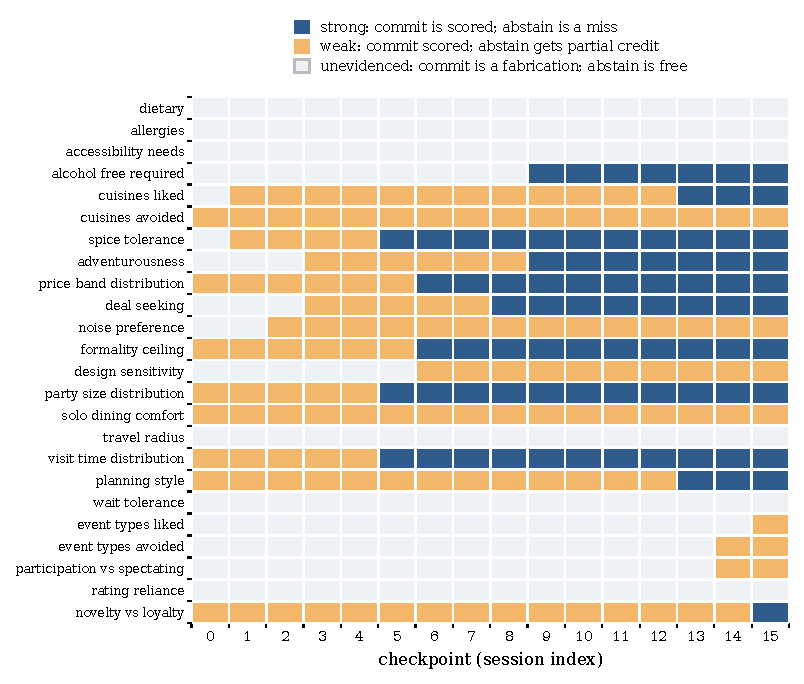
\includegraphics[width=0.62\linewidth]{fig_evidence_map.pdf}
  \caption{The evidence map for one subject (24 fields $\times$ 16 checkpoints, $c_0$--$c_{15}$). No reader credit or
  hand correction changes a grade on this subject, so its bands are exactly the schedule's map
  (\S\ref{sec:map}); each cell is what a careful reader could know so far. Grades never go down, so bands only darken rightward, and the six fields the
  schedule never evidences stay light throughout.}
  \label{fig:map}
\end{figure}

\textbf{Ordinal levels.} Each ordinal field has four discrete levels ($0 \le \ell \le 3$) defined by behaviour, listed here from
lowest ($\mathbf{0}$) to highest ($\mathbf{3}$). Each level is given with the code a system emits
followed by its gloss in the prompts, so that a level is pinned by behaviour in the transcript
rather than by an adjective.
\begin{description}\setlength{\itemsep}{1pt}\small
  \item[\texttt{spice\_tolerance}] \textbf{0}:~\texttt{avoids\_heat} (\emph{avoids heat entirely}) $\to$ \textbf{1}:~\texttt{mild\_only} (\emph{mild only; will ask for it toned down}) $\to$ \textbf{2}:~\texttt{likes\_real\_spice} (\emph{likes real spice and orders for it}) $\to$ \textbf{3}:~\texttt{seeks\_hottest} (\emph{seeks the hottest thing on the menu}).
  \item[\texttt{adventurousness}] \textbf{0}:~\texttt{sticks\_to\_known} (\emph{sticks to dishes they already know}) $\to$ \textbf{1}:~\texttt{familiar\_variations} (\emph{tries variations of the familiar}) $\to$ \textbf{2}:~\texttt{orders\_unfamiliar} (\emph{orders the dish they don't recognize while the table plays safe}) $\to$ \textbf{3}:~\texttt{seeks\_unidentifiable} (\emph{picks the place \emph{because} they can't read the menu}).
  \item[\texttt{deal\_seeking}] \textbf{0}:~\texttt{ignores\_price} (\emph{ignores price}) $\to$ \textbf{1}:~\texttt{notices\_value} (\emph{notices value but doesn't act on it}) $\to$ \textbf{2}:~\texttt{looks\_for\_deals} (\emph{checks for a discount once they have already chosen the place}) $\to$ \textbf{3}:~\texttt{plans\_around\_specials} (\emph{lets the happy-hour window pick the place and the hour}).
  \item[\texttt{noise\_preference}] \textbf{0}:~\texttt{needs\_quiet} (\emph{needs it quiet enough to talk}) $\to$ \textbf{1}:~\texttt{prefers\_low\_hum} (\emph{prefers a low hum}) $\to$ \textbf{2}:~\texttt{fine\_with\_lively} (\emph{fine with lively}) $\to$ \textbf{3}:~\texttt{wants\_loud} (\emph{wants it loud and busy}).
  \item[\texttt{formality\_ceiling}] \textbf{0}:~\texttt{counter\_service} (\emph{counter service only}) $\to$ \textbf{1}:~\texttt{casual\_sit\_down} (\emph{casual sit-down}) $\to$ \textbf{2}:~\texttt{smart\_casual} (\emph{smart-casual}) $\to$ \textbf{3}:~\texttt{white\_tablecloth} (\emph{white tablecloth}).
  \item[\texttt{design\_sensitivity}] \textbf{0}:~\texttt{doesnt\_notice} (\emph{doesn't notice the room}) $\to$ \textbf{1}:~\texttt{mild\_preference} (\emph{mild preference for a nice room}) $\to$ \textbf{2}:~\texttt{room\_matters} (\emph{rules out a place whose room they dislike when there is an alternative}) $\to$ \textbf{3}:~\texttt{room\_over\_food} (\emph{will pick a worse meal for a better room}).
  \item[\texttt{solo\_dining\_comfort}] \textbf{0}:~\texttt{wont\_eat\_alone} (\emph{won't eat alone}) $\to$ \textbf{1}:~\texttt{takeaway\_or\_counter} (\emph{alone only for takeaway or at a counter}) $\to$ \textbf{2}:~\texttt{comfortable\_at\_table} (\emph{comfortable at a table alone}) $\to$ \textbf{3}:~\texttt{enjoys\_solo} (\emph{actively enjoys solo meals}).
  \item[\texttt{travel\_radius}] \textbf{0}:~\texttt{walking\_distance} (\emph{only what they can walk to in ten minutes}) $\to$ \textbf{1}:~\texttt{own\_neighborhood} (\emph{one short bus or subway ride, never across town}) $\to$ \textbf{2}:~\texttt{anywhere\_in\_city} (\emph{will cross the city for it, but not leave it}) $\to$ \textbf{3}:~\texttt{out\_of\_town} (\emph{will get on a train out of town for one meal}).
  \item[\texttt{planning\_style}] \textbf{0}:~\texttt{fully\_spontaneous} (\emph{decides on the pavement, already out}) $\to$ \textbf{1}:~\texttt{decides\_same\_day} (\emph{picks in the morning for that evening}) $\to$ \textbf{2}:~\texttt{books\_days\_out} (\emph{books a few days out}) $\to$ \textbf{3}:~\texttt{books\_weeks\_ahead} (\emph{books weeks ahead}).
  \item[\texttt{wait\_tolerance}] \textbf{0}:~\texttt{leaves\_if\_line} (\emph{turns around if anyone is waiting ahead of them}) $\to$ \textbf{1}:~\texttt{fifteen\_min\_max} (\emph{waits a quarter of an hour, then leaves}) $\to$ \textbf{2}:~\texttt{hour\_for\_the\_right\_place} (\emph{will stand in an hour-long line once they are already there}) $\to$ \textbf{3}:~\texttt{queue\_is\_part\_of\_it} (\emph{plans the evening around being early in the queue; a wait is never a reason to go elsewhere}).
  \item[\texttt{participation\_vs\_spectating}] \textbf{0}:~\texttt{watches\_only} (\emph{watches only}) $\to$ \textbf{1}:~\texttt{joins\_if\_pushed} (\emph{takes part only when asked directly}) $\to$ \textbf{2}:~\texttt{joins\_readily} (\emph{joins in unasked at whatever event they happen to be at}) $\to$ \textbf{3}:~\texttt{seeks\_hands\_on} (\emph{won't book an event where they would only be watching}).
  \item[\texttt{rating\_reliance}] \textbf{0}:~\texttt{ignores\_ratings} (\emph{ignores ratings}) $\to$ \textbf{1}:~\texttt{glances\_at\_them} (\emph{glances at them}) $\to$ \textbf{2}:~\texttt{checks\_before\_going} (\emph{checks ratings before going}) $\to$ \textbf{3}:~\texttt{threshold\_gated} (\emph{won't go below a rating threshold}).
  \item[\texttt{novelty\_vs\_loyalty}] \textbf{0}:~\texttt{same\_few\_places} (\emph{returns to the same few places}) $\to$ \textbf{1}:~\texttt{mostly\_regulars} (\emph{mostly regulars, occasional new}) $\to$ \textbf{2}:~\texttt{mostly\_new} (\emph{mostly new places, some regulars}) $\to$ \textbf{3}:~\texttt{almost\_never\_repeats} (\emph{almost never repeats a venue}).
\end{description}

\textbf{Closed vocabularies for set fields.} A set field's value is any subset of its vocabulary
(the empty set included), and a system may only commit items from the vocabulary.
\begin{description}\setlength{\itemsep}{1pt}\small
  \item[\texttt{dietary}] \texttt{vegetarian}, \texttt{vegan}, \texttt{pescatarian}, \texttt{halal}, \texttt{kosher}, \texttt{gluten\_free}, \texttt{dairy\_free}, \texttt{low\_sodium}, \texttt{keto}.
  \item[\texttt{allergies}] \texttt{peanuts}, \texttt{tree\_nuts}, \texttt{shellfish}, \texttt{fish}, \texttt{eggs}, \texttt{milk}, \texttt{soy}, \texttt{wheat}, \texttt{sesame}.
  \item[\texttt{accessibility\_needs}] \texttt{step\_free\_access}, \texttt{accessible\_restroom}, \texttt{wide\_aisles}, \texttt{low\_lighting\_ok}, \texttt{quiet\_room\_needed}, \texttt{service\_animal}, \texttt{seating\_required}, \texttt{braille\_menu}, \texttt{assistive\_listening}.
  \item[\texttt{cuisines\_liked}, \texttt{cuisines\_avoided}] (39 items, grouped by region/type):
    \begin{itemize}[leftmargin=*, itemsep=0pt, topsep=1pt]
      \item \emph{East \& SE Asian:} \texttt{chinese}, \texttt{dim\_sum}, \texttt{filipino}, \texttt{japanese}, \texttt{korean}, \texttt{malaysian}, \texttt{ramen}, \texttt{sushi}, \texttt{taiwanese}, \texttt{thai}, \texttt{vietnamese}.
      \item \emph{European \& Mediterranean:} \texttt{french}, \texttt{german}, \texttt{greek}, \texttt{italian}, \texttt{mediterranean}, \texttt{moroccan}, \texttt{portuguese}, \texttt{spanish}, \texttt{turkish}.
      \item \emph{Americas \& Casual:} \texttt{american}, \texttt{bbq}, \texttt{burgers}, \texttt{cajun}, \texttt{caribbean}, \texttt{deli}, \texttt{latin\_american}, \texttt{mexican}, \texttt{peruvian}, \texttt{soul\_food}, \texttt{steakhouse}.
      \item \emph{South Asian, Middle Eastern, African \& Other:} \texttt{brunch}, \texttt{ethiopian}, \texttt{indian}, \texttt{lebanese}, \texttt{middle\_eastern}, \texttt{pizza}, \texttt{seafood}, \texttt{vegan\_restaurant}.
    \end{itemize}
  \item[\texttt{event\_types\_liked}, \texttt{event\_types\_avoided}] \texttt{art\_opening}, \texttt{book\_reading}, \texttt{comedy}, \texttt{cooking\_class}, \texttt{dance\_night}, \texttt{film\_screening}, \texttt{food\_festival}, \texttt{karaoke}, \texttt{live\_jazz}, \texttt{live\_rock}, \texttt{market}, \texttt{museum\_late}, \texttt{open\_mic}, \texttt{pub\_quiz}, \texttt{supper\_club}, \texttt{tasting\_menu}, \texttt{theater}, \texttt{wine\_tasting}.
\end{description}

\textbf{Distribution bins.} \texttt{price\_band\_distribution} is over per-head spend
($<$\pounds15, \pounds15--30, \pounds30--50, \pounds50+); \texttt{party\_size\_distribution} over
party size (1, 2, 3--5, 6+); \texttt{visit\_time\_distribution} over occasion (weekday lunch,
weekday evening, weekend day, weekend evening, late night). A distribution is kept, rather than
the single most common bin, because it preserves two-peaked behaviour (cheap weeknights and
occasional blowouts) that a single value would flatten.

\textbf{Reader credit and hand corrections in numbers.} The reader credit of \S\ref{sec:map}
raises 181 cells in 28 subjects from \textsc{unevidenced} to \textsc{weak} (170 on both evidence
readers, 11 on one and a human ruling) and lowers none. The hand corrections leave 44 cells in 9
subjects different from the schedule's grade (29 raised to \textsc{weak}, 15 lowered to
\textsc{unevidenced}), and correct 86 gold-card values in 45 subjects, 67 of them by removing a
list item the transcript never voiced.

\phantomsection\label{app:example}
\textbf{A worked example.} The first session of subject \texttt{gen-000} opens: ``\emph{Looking
for somewhere to eat tonight, just me. Not planning on spending much --- under fifteen quid
ideally.} [\dots] \emph{Somewhere I can just order at the counter} [\dots] \emph{I just don't want
to be crossing the whole city for it.}'' Its one beat (the last line, a reaction) makes
\texttt{travel\_radius} \textsc{weak}. Its occasion (a party of one, under \pounds15, a weekend
evening) makes the three distributions \textsc{weak} (too few occasions to score yet,
\S\ref{sec:scoring}) and, as implied traits, \texttt{solo\_dining\_comfort},
\texttt{formality\_ceiling} (a counter-service outing, credited because counter service is this
subject's ceiling; an outing below a subject's ceiling credits nothing, so the same request is a
fabrication in the subjects of \S\ref{sec:failures}) and \texttt{planning\_style} (a same-day
plan). The other 17 fields stay \textsc{unevidenced} at $c_0$, including \texttt{spice\_tolerance},
whose gold value is \texttt{seeks\_hottest}: committing it here is a fabrication even though it is
right.

% ===========================================================================
\section{The zero-cost baselines}
\label{app:gate}
% ===========================================================================

Table~\ref{tab:gate} gives the four zero-cost baselines of \S\ref{sec:scoring} in full. None of the four
reads a transcript, so their values are fixed by construction and are
run before any model as a check on the key and harness. The \texttt{oracle} commits the gold value on
every field the map grades \textsc{strong} or \textsc{weak} and abstains elsewhere; \texttt{abstain}
emits \texttt{unknown} on every field; \texttt{population} commits the most common value in the
corpus on every field at every checkpoint; \texttt{random} commits a value drawn uniformly at random.
Skill is fidelity rescaled at each checkpoint so that \texttt{abstain} $=0$ and \texttt{oracle}
$=1$, then averaged over eligible checkpoints (\S\ref{sec:scoring}), so the first two rows are the
anchors themselves.

The oracle's fidelity is exactly $1.000$ at every checkpoint of every subject, so the gold card and
the map agree. Both always-committing baselines fabricate on the same 3,908 cells, which is every
\textsc{unevidenced} preference-field cell at any checkpoint, and at $\lambda=1$ both land near
skill $-4$. \texttt{abstain} has a hard-constraint failure rate of $0.56$ because an
\texttt{unknown} on an evidenced constraint field with a non-empty gold value counts as a miss
(\S\ref{sec:scoring}).

\begin{table}[h]
  \centering
  \caption{The zero-cost baselines fix the scorer's ceiling and floor. All 50 subjects (612 sessions); 47
  enter the AUFC and skill means (\S\ref{sec:scoring}). All four values are fixed by construction.
  Both always-committing baselines lose to silence.}
  \label{tab:gate}
  \begin{tabular}{@{}lrrrr@{}}
    \toprule
    Baseline & mean AUFC & skill & fabrications & hard-constraint failure rate \\
    \midrule
    \texttt{oracle} (ceiling)     & \textbf{1.000} & 1.000  & 0    & 0.00 \\
    \texttt{abstain} (floor)      & 0.629 & \textbf{0.000} & 0    & 0.56 \\
    \texttt{population}           & 0.117 & $-3.969$ & 3,908 & 0.56 \\
    \texttt{random}               & 0.114 & $-3.943$ & 3,908 & 1.00 \\
    \bottomrule
  \end{tabular}
\end{table}

% ===========================================================================
\section{Skill by system and backbone}
\label{app:resultstable}
% ===========================================================================

Table~\ref{tab:results} gives the numbers plotted in Figure~\ref{fig:results}, plus the single
stateful cell reported in the text of \S\ref{sec:results}, over the same subjects.

\textbf{Paired comparisons.} Gaps are tested in AUFC, not in the skill the table reports, by a
paired bootstrap over subjects; $\Delta\mathrm{AUFC}$ is the first system's AUFC minus the
second's, and the intervals are 95\%. Each gap is also recomputed under all 27 combinations of
$\lambda\in\{0.5,1,2\}$, \textsc{weak-credit} $\in\{\nicefrac{5}{6}-0.08,\nicefrac{5}{6},\nicefrac{5}{6}+0.08\}$,
and an eligibility threshold of $5$, $7$, or $10$ evidenced fields.
\begin{itemize}
  \item Gemini 3.7 Flash, \texttt{prompted} $-$ \texttt{notebook}: $+0.009$, CI $[+0.001, +0.017]$;
  \texttt{prompted} is ahead under all 27 settings.
  \item GLM-5.3 Flash, \texttt{prompted} $-$ \texttt{notebook}: $+0.015$, CI $[-0.005, +0.034]$;
  borderline.
  \item GPT-5.6 Luna and DeepSeek V4 Pro, \texttt{prompted} $-$ \texttt{notebook}: the intervals
  straddle zero and the sign changes across settings.
  \item GPT-5.6 Luna, \texttt{memory} $-$ \texttt{prompted}: $-0.065$, CI $[-0.084, -0.044]$;
  \texttt{memory} $-$ \texttt{notebook}: $-0.067$, CI $[-0.082, -0.052]$; both hold under every
  setting.
\end{itemize}

\begin{table}[h]
  \centering
  \caption{Skill (fidelity rescaled per checkpoint so \texttt{abstain} $=0$, \texttt{oracle} $=1$; \S\ref{sec:scoring}) by system and
  backbone, all 50 subjects. Higher is better; negative is
  worse than emitting nothing. The single-pass systems clear the floor by a wide margin on every
  backbone. The stateful system (\texttt{memory}) is scored on GPT-5.6 Luna only; the other three
  cells are unrun.}
  \label{tab:results}
  \begin{tabular}{@{}lcccc@{}}
    \toprule
    System & Gemini 3.7 Flash & GPT-5.6 Luna & DeepSeek V4 Pro & GLM-5.3 Flash \\
    \midrule
    \texttt{prompted}          & $+0.813$ & $+0.669$ & $+0.590$ & $+0.497$ \\
    \texttt{notebook}          & $+0.789$ & $+0.700$ & $+0.601$ & $+0.434$ \\
    \texttt{memory}            & ---      & $+0.493$ & ---      & ---      \\
    \bottomrule
  \end{tabular}
\end{table}

% ===========================================================================
\section{The three systems under test}
\label{app:suts}
% ===========================================================================

Figure~\ref{fig:suts} draws one checkpoint of each system of \S\ref{sec:results}. Every system
receives the same input at a checkpoint (the new sessions since the last checkpoint, never the
earlier ones) and must emit a full persona card. What differs is the number of model calls
spent and what is carried forward (the cylinders), which is the only thing the system sees of its own
past at the next checkpoint. All three systems also carry a running count of occasions for the three
distribution fields. The model reports one bin per occasion it sees, the code adds them up, and the
card's distributions are the normalised counts, so a distribution is built from counted occasions
rather than re-estimated from memory.

\begin{figure}[h]
  \centering
  \tikzset{
    llm/.style={draw, rounded corners, align=center, inner sep=2pt,
                minimum height=6mm, minimum width=15mm, fill=black!8, font=\scriptsize},
    io/.style={align=center, font=\scriptsize\itshape, inner sep=1pt, text width=15mm},
    store/.style={draw, cylinder, shape border rotate=90, aspect=0.22, align=center,
                  inner sep=1.5pt, fill=black!4, font=\tiny, minimum width=15mm, minimum height=6mm},
    a/.style={-{Latex[length=1.5mm]}, semithick},
    ad/.style={-{Latex[length=1.5mm]}, semithick, densely dashed},
    carry/.style={font=\tiny\itshape, inner sep=1pt},
  }
  %--- (a) prompted -------------------------------------------------------
  \begin{subfigure}[b]{0.31\linewidth}
    \centering
    \begin{tikzpicture}[node distance=4mm]
      \node[io] (in) {new sessions};
      \node[llm, below=of in] (llm) {emit};
      \node[io, below=of llm] (out) {card};
      \node[store, below=of out] (st) {card};
      \draw[a] (in) -- (llm);
      \draw[a] (llm) -- (out);
      \draw[ad] (out) -- (st);
      \draw[ad] (st.east) -- ++(4mm,0) |- (llm.east);
    \end{tikzpicture}
    \caption{\texttt{prompted}}
    \label{fig:sut-prompted}
  \end{subfigure}\hfill
  %--- (b) notebook -------------------------------------------------------
  \begin{subfigure}[b]{0.31\linewidth}
    \centering
    \begin{tikzpicture}[node distance=4mm]
      \node[io] (in) {new sessions};
      \node[llm, below=of in] (llm) {emit};
      \node[io, below=of llm] (out) {card};
      \node[store, below=of out, minimum width=17mm] (st) {card + notes};
      \draw[a] (in) -- (llm);
      \draw[a] (llm) -- (out);
      \draw[ad] (out) -- (st);
      \draw[ad] (st.east) -- ++(4mm,0) |- (llm.east);
    \end{tikzpicture}
    \caption{\texttt{notebook}}
    \label{fig:sut-notebook}
  \end{subfigure}\hfill
  %--- (c) memory ---------------------------------------------------------
  \begin{subfigure}[b]{0.31\linewidth}
    \centering
    \begin{tikzpicture}[node distance=4mm]
      \node[io] (in) {new sessions};
      \node[llm, below=of in] (e) {extract};
      \node[io, below=of e] (cand) {candidates};
      \node[llm, below=of cand] (i) {integrate};
      \node[io, below=of i] (out) {card};
      \node[store, below=of out] (st) {bank};
      \draw[a] (in) -- (e);
      \draw[a] (e) -- (cand);
      \draw[a] (cand) -- (i);
      \draw[a] (i) -- (out);
      \draw[ad] (i.east) -- ++(4mm,0) |- (st.east);
      \draw[ad] (st.west) -- ++(-4mm,0) |- (i.west);
    \end{tikzpicture}
    \caption{\texttt{memory}}
    \label{fig:sut-memory}
  \end{subfigure}
  \caption{The three systems under test, one checkpoint each (input \emph{new sessions} on top,
  emitted \emph{card} on the bottom). Boxes are model calls. Cylinders are carried
  state (dashed loops), the only thing a system sees at the next checkpoint since earlier sessions
  are never re-served. The single-pass pair (\subref{fig:sut-prompted},~\subref{fig:sut-notebook})
  spend one call and carry the last card (\texttt{notebook} also its notes); \texttt{memory}~(\subref{fig:sut-memory}) spends two,
  one to extract and one to integrate, and carries an explicit bank the card is re-read from.}
  \label{fig:suts}
\end{figure}

\textbf{\texttt{prompted}} (\subref{fig:sut-prompted}) is one call. The model is shown the card it
emitted at the previous checkpoint and the new sessions, and emits the card again. Beyond the
occasion counts, its carried state is that card alone. Anything it wants to keep must therefore live in a card field; there is nowhere else to put it.

\textbf{\texttt{notebook}} (\subref{fig:sut-notebook}) is the same loop with one addition: a
free-text scratchpad the model writes at each checkpoint and is shown back at the next, alongside
the last card. It uses the same call budget as \texttt{prompted} with more carried state, and tests
whether free-form carried notes (reminders of weak evidence, context that does not fit a field) buy
anything over the card alone.

\textbf{\texttt{memory}} (\subref{fig:sut-memory}) is two calls with a deliberate information
barrier between them. The \emph{extract} call reads only the new sessions and writes candidate
memories; it never sees the bank, so it cannot rubber-stamp ``nothing changed.'' The \emph{integrate}
call is shown the bank and the candidates, never the raw conversation. It decides for each
candidate whether to add it, let it supersede an existing entry, or drop it as a duplicate, and then
rebuilds the card from the updated bank. The carried state is the bank, plus the occasion counts,
which grow from the extract call because it is the only one that reads the conversation. The handoff between the
two calls loses information by design: whatever the extractor fails to write down is gone. That
loss is the cost this system exists to measure. In our run it explains the starved distributions;
most of the stateful failures of \S\ref{sec:failures} come instead from the integrate call, which
re-reads the card from the bank afresh at every checkpoint.

All three are reference implementations run on fixed system prompts, which are reproduced in Appendix~\ref{app:prompts} and ship with the benchmark.

\textbf{Backbones and routing.} All four backbones are called through OpenRouter at the fixed
routes of Table~\ref{tab:backbones}. DeepSeek V4 Pro and GLM-5.3 Flash are pinned to one provider
with fallbacks off, so every call hits the same endpoint; GPT-5.6 Luna and Gemini 3.7 Flash route by
OpenRouter default. We send no reasoning-effort override, so the effort shown is each route's
OpenRouter default, not a setting we chose. Every model in this paper, the four backbones and the
Claude models that build the corpus and read the failures, is used through its provider's API under
the provider's terms of use.

\begin{table}[h]
  \centering
  \caption{Backbone routing. All calls go through OpenRouter. \emph{Effort} is the route's
  OpenRouter default; \emph{Reasoning} is whether chain-of-thought is on at
  that default, which we did not verify for DeepSeek V4 Pro.}
  \label{tab:backbones}
  \footnotesize
  \setlength{\tabcolsep}{4pt}
  \begin{tabular}{@{}lllll@{}}
    \toprule
    Backbone & OpenRouter route & Provider & Effort & Reasoning \\
    \midrule
    Gemini 3.7 Flash & \texttt{google/gemini-3.7-flash}        & OpenRouter default    & \texttt{medium} & always on \\
    GPT-5.6 Luna     & \texttt{openai/gpt-5.6-luna}            & OpenRouter default    & \texttt{medium} & on by default \\
    DeepSeek V4 Pro  & \texttt{deepseek/deepseek-v4-pro-0813}  & Alibaba, no fallback  & \texttt{high}   & not verified \\
    GLM-5.3 Flash    & \texttt{z-ai/glm-5.3-flash}             & Z.AI fp8, no fallback & \texttt{max}    & always on \\
    \bottomrule
  \end{tabular}
\end{table}

% ===========================================================================
\section{System prompts}
\label{app:prompts}
% ===========================================================================

The three systems of Appendix~\ref{app:suts} run on the system prompts below, reproduced verbatim
from the released code. Each was
written from the schema and the answer key's evidence policy. \texttt{prompted} and \texttt{notebook} share one system prompt
(\S\ref{app:prompt-card}); \texttt{memory} has one per call (\S\ref{app:prompt-extract},
\S\ref{app:prompt-integrate}). The per-checkpoint user turn differs by call. The single-pass calls
get the 24-field menu with each value's gloss and bins (Appendix~\ref{app:fields}), the last card
(for \texttt{notebook} also its notes), the new sessions, an instruction to report the three
distribution fields as one data point per occasion seen in the new sessions rather than as estimated
shares, and the JSON shape to emit. \texttt{memory}'s extract call gets only the new sessions, the
same data-point instruction, and the JSON shape; it is never shown the field menu
(\S\ref{sec:failures}). The integrate call gets the field menu, the bank, and the new candidates, and leaves the
distribution fields to the counted data points.

\Needspace{8\baselineskip}
\subsection{\texttt{prompted} and \texttt{notebook}}
\label{app:prompt-card}
{\nolinenumbers
\begin{lstlisting}
You are building a preference profile of one person from their conversations with a restaurant-recommendation assistant. You will be shown their conversations a few at a time, in order, and after each batch you output the profile as it stands.

You are scored on CALIBRATION, not on coverage. For each field:

  - the conversations so far PIN the value  -> give the value. Saying "unknown" scores zero.
  - the conversations so far NARROW it      -> give your best value. "unknown" gets partial credit.
  - the conversations have NOT TOUCHED it   -> say "unknown". A value here is a FABRICATION and is penalised EVEN IF IT HAPPENS TO BE CORRECT.

That last line is the whole task. Guessing from a stereotype, from a population base rate, or from another field ("they like Sichuan, so they must want it hot") earns nothing and costs you whenever the conversations have not shown it. This dataset deliberately contains people who violate the usual correlations, so the guess is not even reliably right.

Seven fields hold LISTS: dietary, allergies, accessibility_needs, cuisines_liked, cuisines_avoided, event_types_liked, event_types_avoided. On these, an empty list [] is NOT the same as "unknown": it is a positive claim that the person has NONE, scored as a commitment, so on a field the conversations have not established it is a FABRICATION. Two rules:

  - dietary, allergies, accessibility_needs: write [] ONLY once the person has said they have none ("no allergies", "no dietary needs"). Until they do, say "unknown".
  - cuisines_liked, cuisines_avoided, event_types_liked, event_types_avoided: never write [] -- say "unknown" when nothing has been shown, otherwise list what they have shown.

What counts as evidence about this person:

  - only what the PERSON says, orders, chooses or rejects. What the ASSISTANT offers, describes or assumes is scenery, even about a place the person then books.
  - booking a venue is not liking its cuisine or format. If they took it for the distance, the quiet room, the price or the availability, the cuisine in the assistant's description is NOT evidenced -- only the person naming or ordering the cuisine themselves is.
  - a FRIEND, PARTNER or COLLEAGUE's needs are theirs, not this person's. A companion's nut allergy is not a nut allergy here.
  - a claim about themselves that their behaviour contradicts. Record what they DO.
  - a CEILING field (formality_ceiling: the highest formality they will go to) is an upper bound. Asking for or accepting something BELOW it says nothing about where the bound sits; only the highest level they have actually gone to evidences it.
  - use the level whose words they used, not a neighbour: sushi is not japanese, a market is not a food_festival.

Output JSON only, no prose outside it.
\end{lstlisting}}

\Needspace{8\baselineskip}
\subsection{\texttt{memory}: extract call}
\label{app:prompt-extract}
{\nolinenumbers
\begin{lstlisting}
You are reading someone's conversations with a restaurant-recommendation assistant and writing down what you learn about them, as durable memory items you can consult later without ever re-reading this conversation.

Write each memory as one atomic, self-contained sentence, with enough of its own evidence baked in that a later reader who never sees this conversation can judge how strong it is. Prefer "they said directly: ..." over a paraphrase that hides whether it was stated, implied, or merely consistent with what they ordered.

What a memory about this person may record:

  - only what the PERSON said, ordered, chose or rejected. What the ASSISTANT offered, described or assumed is scenery, even about a place the person then booked -- if you record the booking, record the reason they gave, and mark any cuisine or format as the assistant's description, not theirs.
  - booking a venue is not liking its cuisine or format. Taken for the distance, the quiet room, the price or the availability, it evidences nothing about the cuisine; only the person naming or ordering the cuisine themselves does.
  - a FRIEND, PARTNER or COLLEAGUE's needs are theirs, not this person's. A companion's nut allergy is not a nut allergy here.
  - a claim about themselves their behaviour contradicts. Write what they DID, and say so if it conflicts with something they claimed.
  - asking for or accepting something BELOW a ceiling (formality_ceiling: the highest formality they will go to) says nothing about where the ceiling sits. Record the highest level they actually went to, not every level below it.
  - record the words they used, not a neighbour: sushi is not japanese, a market is not a food_festival.

Skip small talk and anything that reveals nothing about their preferences, habits or constraints.
A conversation with nothing durable in it can produce zero memories -- that is a correct output,
not a failure.

Output JSON only, no prose outside it.
\end{lstlisting}}

\Needspace{8\baselineskip}
\subsection{\texttt{memory}: integrate call}
\label{app:prompt-integrate}
{\nolinenumbers
\begin{lstlisting}
You maintain one person's preference profile from a running memory bank, built from their conversations with a restaurant-recommendation assistant. You do not see the conversations themselves -- only the memory items already on file and the new candidates just written from the latest ones. You are scored on CALIBRATION, not on coverage. For each tracked field:

  - the memories on file PIN the value   -> give the value. Saying "unknown" scores zero.
  - the memories NARROW it               -> give your best value. "unknown" gets partial credit.
  - no memory touches it                 -> say "unknown". A value here is a FABRICATION and is penalised EVEN IF IT HAPPENS TO BE CORRECT.

Guessing from a stereotype, a population base rate, or another field earns nothing and costs you whenever no memory on file supports it.

Seven fields hold LISTS: dietary, allergies, accessibility_needs, cuisines_liked, cuisines_avoided, event_types_liked, event_types_avoided. On these, an empty list [] is NOT the same as "unknown": it is a positive claim that the person has NONE, scored as a commitment, so on a field no memory on file establishes it is a FABRICATION. Two rules:

  - dietary, allergies, accessibility_needs: write [] ONLY once a memory on file says they have none ("no allergies", "no dietary needs"). Until one does, say "unknown".
  - cuisines_liked, cuisines_avoided, event_types_liked, event_types_avoided: never write [] -- say "unknown" when no memory shows any, otherwise list what the memories support.

What a memory on file licenses:

  - only what the PERSON said, ordered, chose or rejected. A memory of what the ASSISTANT offered, described or assumed licenses nothing, even about a place the person booked.
  - booking a venue is not liking its cuisine or format. A memory that they took a venue the assistant called Mediterranean, for the distance, the quiet room, the price or the availability, does not put mediterranean in cuisines_liked; only a memory of the person naming or ordering the cuisine does.
  - a FRIEND, PARTNER or COLLEAGUE's needs are theirs, not this person's.
  - a CEILING field (formality_ceiling: the highest formality they will go to) is an upper bound. A memory of a request or a booking BELOW it says nothing about where the bound sits; only the highest level on file evidences it.
  - use the level whose words the memory records, not a neighbour: sushi is not japanese, a market is not a food_festival.

You also maintain the memory bank itself. For every new candidate below, decide exactly one of:

  - "add"       - genuinely new information; keep it as its own item.
  - "supersede" - it updates or corrects an item already on file; name that item's id in "supersedes" -- the old item is dropped in favour of the new text. A person who says they have stopped eating meat has changed, and the bank should change with them.
  - "duplicate" - it says nothing the bank does not already have; it is dropped.

Output JSON only, no prose outside it.
\end{lstlisting}}

% ===========================================================================
\section{Failure-mode catalogue}
\label{app:failures}
% ===========================================================================

This appendix backs \S\ref{sec:failures} with the procedure, the numbers behind each claim, and the
caveats that attach to them.

\textbf{Runs.} The catalogue covers the nine runs of \S\ref{sec:results}, each on every
checkpoint of all 50 subjects: \texttt{prompted} and \texttt{notebook} on all four backbones
(Gemini 3.7 Flash, GPT-5.6 Luna, DeepSeek V4 Pro, GLM-5.3 Flash), and \texttt{memory} on
GPT-5.6 Luna.

\textbf{Procedure.} The catalogue is built in five steps.
\begin{enumerate}[leftmargin=*, itemsep=1pt, label=(\arabic*)]
  \item \emph{Recover the charged cells.} Every cell the scorer charged (a committed preference
  scoring below $0.5$, a fabrication, or a missed or invented constraint element) is recovered by replaying
  the cached outputs against the answer key.
  \item \emph{Group them into episodes.} Cells are grouped by (system, backbone, subject, field,
  element); a new episode opens when checkpoints are not consecutive or the emitted value changes.
  This gives 807 episodes.
  \item \emph{Read each distinct case once.} Episodes collapse to distinct cases
  (subject, field, element, emitted value, gold value, first checkpoint); what the transcript
  supports at a checkpoint does not depend on which system emitted the value, so each case is read
  once and its verdict applies to every episode in it. Failure readers (Claude Opus~5.5, shown neither
  the system nor any earlier verdict) read the
  full served transcript and label each case \textsc{genuine}, \textsc{key artifact}, or
  \textsc{ambiguous} under the answer key's evidence policy, with a supporting quote, the failure
  mode, and a flag where the reader doubted the gold.
  \item \emph{Read every non-genuine case again.} The 76 cases not labelled \textsc{genuine} were read
  a second time by independent failure readers who did not see the first verdict. Where the two reads
  disagreed, a first-read \textsc{ambiguous} that the second read called \textsc{genuine} is taken
  as \textsc{genuine}; the rest were settled from the run data or by the authors.
  \item \emph{Correct the key where it was wrong, and tally.} The reading was first done against the
  key before its last correction. The failure readers found the key wrong on four fields there: three
  deal-seeking fields and one avoided cuisine were graded evidenced too late (two) or with no user
  line behind them (two). Those four are corrected in the released key, the
  episodes were re-extracted against it, and the three cases that changed were read afresh (all
  \textsc{genuine}). Final mix on the 807 episodes: 742 \textsc{genuine} (92\%), 60
  \textsc{key artifact} (7.4\%), 5 \textsc{ambiguous}. The key artifacts have three causes: 37
  episodes (4.6\%) are the system recording what the user said under a neighbouring label (a wheat
  allergy filed as \texttt{gluten\_free}), 21 (2.6\%) are a safe default on a field never raised
  (\texttt{alcohol\_free\_required} false, an empty list), and 2 (0.2\%) are the gold itself being
  wrong, in two \emph{visit-time} distributions whose hidden histogram disagrees with the visits the
  transcript shows. These two are left as they are: every distribution is scored against the final
  card (\S\ref{sec:scoring}), and re-keying these two to the visits shown would make them the only
  distributions keyed that way.
\end{enumerate}
Every number in \S\ref{sec:failures} is on \textsc{genuine} episodes, the ``confirmed mistakes'' of
that section.

\textbf{Caveats.}
\begin{enumerate}[leftmargin=*, itemsep=1pt, label=(\roman*)]
  \item \emph{The failure readers are LLMs.} They apply a written policy and are not human annotators. A
  case the first read called \textsc{genuine} was not read again, so most of the \textsc{genuine} count
  (440 of 472 cases) rests on one read.
  \item \emph{One stateful run.} The stateful mechanism (an unstable re-read, contradictions added
  rather than superseding, bins starved of data) is read from \texttt{memory} on one backbone.
  \item \emph{Undisclosed rule.} Some turns show an abstract trait (participation, spice) in loose
  words. The prompts do not tell systems that such a turn supports only that trait, so that every
  backbone falls for it reflects the prompt as much as the backbone.
\end{enumerate}

\begin{table}[h]
  \centering
  \caption{Confirmed mistakes per subject on the nine runs (all 50 subjects).
  ``---'' = run not made. Backbone choice outweighs the scratchpad: the same system spreads by up to
  $2.3$ per subject across backbones (seven-fold), against at most $0.6$ for the notes
  scratchpad.}
  \label{tab:fail-runs}
  \small
  \begin{tabular}{@{}lccc@{}}
    \toprule
    Backbone & \texttt{prompted} & \texttt{notebook} & \texttt{memory} \\
    \midrule
    Gemini 3.7 Flash & 0.38 & 0.42 & --- \\
    GPT-5.6 Luna     & 0.90 & 0.84 & 3.14 \\
    DeepSeek V4 Pro  & 2.66 & 2.04 & --- \\
    GLM-5.3 Flash    & 2.10 & 2.36 & --- \\
    \bottomrule
  \end{tabular}
\end{table}

\begin{table}[h]
  \centering
  \caption{Share of each backbone's confirmed mistakes by mode (single-pass, both systems pooled,
  all 50 subjects). \emph{Unevidenced}: a commit on a field not yet evidenced, split by whether the
  value happens to match the hidden one (\emph{lucky}) or not. \emph{List}: a committed list that
  is a strict superset or subset of the gold. \emph{Constraint}: an invented or missed element of a
  hard-constraint field. \emph{Ordinal}: a value two or more levels off. Rows do not sum to
  100\%; the remainder falls in modes not shown. Shares are rounded separately.}
  \label{tab:fail-profile}
  \small
  \begin{tabular}{@{}lrrrrrrrr@{}}
    \toprule
    & & \multicolumn{2}{c}{Unevidenced} & \multicolumn{2}{c}{List} & \multicolumn{2}{c}{Constraint}
      & Ordinal \\
    \cmidrule(lr){3-4} \cmidrule(lr){5-6} \cmidrule(lr){7-8} \cmidrule(l){9-9}
    Backbone & $n$ & wrong & lucky & superset & subset & invented & missed & ${\ge}2$ off \\
    \midrule
    Gemini 3.7 Flash & 40  & 60\% & 2\%  & 0\%  & \textbf{18\%} & 0\%  & 10\% & 0\% \\
    GPT-5.6 Luna     & 87  & 54\% & 6\%  & 3\%  & 6\%  & 8\%  & 6\%  & 9\% \\
    DeepSeek V4 Pro  & 235 & 45\% & 5\%  & 1\%  & 3\%  & \textbf{30\%} & 6\% & 5\% \\
    GLM-5.3 Flash    & 223 & \textbf{65\%} & 10\% & 2\% & 2\% & 8\% & 2\% & 8\% \\
    \bottomrule
  \end{tabular}
\end{table}

\textbf{Early commits.} For each fabrication episode, \emph{lead} is the number of checkpoints
between the commit and the field's first evidenced checkpoint. Across the single-pass runs
the median lead, where finite, is 2--4 checkpoints; 23--45\% of fabrications are on a field never
evidenced in the subject; the committed value is contained in the final gold in 0--17\% of episodes
(Gemini 3.7 Flash \texttt{prompted} 0/13, GLM-5.3 Flash \texttt{notebook} 14/87, GPT-5.6 Luna
\texttt{prompted} 5/29); and the ``lucky'' share of all fabrications is 0--16\% on every run.
Fabrications start early for single-pass systems (median 0.11 of the way through the conversation,
45\% at $c_0$) and later for the stateful one (0.43, 9\%).

\textbf{Ordinal fields.} 266 of 323 ordinal errors are commits on a field graded unevidenced.
Most common guesses on a field not yet evidenced, pooled over the backbones: \emph{deal-seeking}
\texttt{notices\_value} 87\%;
\emph{noise} \texttt{fine\_with\_lively} 100\%; \emph{design} split between the two middle
levels \texttt{mild\_preference} and \texttt{room\_matters} (13/9);
\emph{formality ceiling} \texttt{casual\_sit\_down} 65\% / \texttt{counter\_service} 30\%;
\emph{adventurousness} \texttt{orders\_unfamiliar} 41\%.
The most common confusions (emitted $\to$ gold) are \texttt{notices\_value}$\to$\texttt{plans\_around\_specials} ($\times$47),
\texttt{notices\_value}$\to$\texttt{looks\_for\_deals} ($\times$28),
\texttt{casual\_sit\_down}$\to$\texttt{white\_tablecloth} ($\times$27), and
\texttt{casual\_sit\_down}$\to$\texttt{smart\_casual} ($\times$17).

\textbf{Shared triggers.} Independent failure readers arrived at the same list; it gives
each trigger, a verbatim example, and who falls for it.
\begin{description}\setlength{\itemsep}{1pt}\small
  \item[Budget cap $\to$ deal-seeking.] ``Nothing over fifteen quid if I can help it'' ($c_0$) $\to$
  \texttt{notices\_value} from seven of the nine runs, on three backbones (Gemini 3.7 Flash is the
  exception). The single most repeated error line in the catalogue.
  \item[Ceiling from the first occasion.] ``Somewhere we sit up at a counter and order as we go'' ($c_0$)
  $\to$ \texttt{formality\_ceiling}=\texttt{counter\_service} from five of the nine runs, on all four
  backbones; the true ceiling
  surfaces at $c_2$ (``I'll be in a jacket''). On Gemini 3.7 Flash and GLM-5.3 Flash
  \texttt{notebook} the prompt's own ceiling clause becomes the reason to commit at $c_0$
  (``highest formality actually gone to is casual sit-down'', gold \texttt{white\_tablecloth}).
  \item[Abstract turn read as a concrete event.] A turn written to evidence participation or spice is re-read as a concrete
  event or a nearby trait: ``me watching it happen'' $\to$ \texttt{live\_jazz} avoided by eight
  of the nine runs; ``we went to a wine thing \ldots\ I was climbing the walls'' $\to$
  \texttt{wine\_tasting} avoided by eight. One of two triggers every backbone falls for on both single-pass
  systems; the other, a format turned into an event type (below), is the largest single source of
  invented event types.
  \item[Soft preference $\to$ hard constraint.] ``Quiet enough to hear myself think'' $\to$
  \texttt{quiet\_room\_needed}; ``a proper table rather than perching'' $\to$
  \texttt{seating\_required} ($\times$74 across runs, DeepSeek V4 Pro $\times$55; \texttt{quiet\_room\_needed}
  $\times$22, 16 of them DeepSeek V4 Pro \texttt{prompted}, which files the request beside the
  correct \texttt{needs\_quiet} after the user has said ``no access requirements, stairs are fine'').
  DeepSeek V4 Pro, GLM-5.3 Flash, GPT-5.6 Luna, and the stateful run; \emph{accessibility needs} is
  the single hottest field (165 episodes).
  \item[A one-off situation read as a trait.] ``We're twenty minutes out'' $\to$ \emph{travel radius}
  (five runs, three backbones); ``watching the clock'' $\to$ \texttt{watches\_only}.
  \item[A format turned into an event type.] A food hall chosen or praised as a format becomes
  \texttt{market}, the most-invented event type ($\times$44: 35 as liked, 9 as avoided; on all nine runs), with the user's own
  word ``market'' in the transcript before onset in most of them; the most common guess on a
  never-raised event field for every backbone. The prompt's ``use the level whose words they used''
  is read as literal word-matching (``The market. I went to one of those'' $\to$ \texttt{market}).
  \item[Booking $\neq$ liking / assistant label copied.] A venue the assistant offered, booked for a
  side reason (a quiet room, a wheat-free kitchen, its hours), enters \emph{cuisines liked} in the
  assistant's word (``Javanese and Malay food'' $\to$ \texttt{malaysian}). The prompt states this
  policy to the systems and it largely holds: 31 episodes over nine runs invent a liked cuisine, and
  the most-invented one (\texttt{burgers}, $\times$12) comes from the user's own words, not the
  assistant's.
\end{description}

\textbf{Agreement across backbones.} For \texttt{prompted} (four backbones), 177
distinct (subject, field) cells (a constraint field split by item) fail; 114 (64\%) under one backbone, 42 under two, 13 under three,
8 (5\%) under all four. \texttt{notebook}: 163 cells, 64\% / 6\%.

\textbf{Whole-card wipes.} The wipe counts of \S\ref{sec:failures} are taken from the raw cached
outputs of all eight single-pass runs. Nothing in the wiped batches contradicts what was held:
eight of DeepSeek V4 Pro \texttt{prompted}'s sixteen wipe sessions contain no dining event at all.
On that run, 9 held constraints are never recovered (e.g.\ \texttt{alcohol\_free\_required} held $c_5$--$c_{26}$,
gone $c_{27}$--$c_{29}$). A scratchpad protects a value only when it restates it, which is why
DeepSeek V4 Pro wipes less under \texttt{notebook} than under \texttt{prompted} (6 against 16); a
note that only says ``no new evidence'' does not protect the next checkpoint.

\textbf{Stateful mechanism.} Beside the loss and flicker shares of \S\ref{sec:failures},
47\% of \texttt{memory}'s episodes are over-reach, against 67--76\% for the single-pass systems on
GPT-5.6 Luna; across all eight single-pass runs, 0--6\% of wrong cells flicker. Of seven flickering cells
traced through the raw outputs of the two calls, five are the card being re-read differently from an
\emph{unchanged} bank (one accessibility item written once yields a card that alternates between two
readings thirteen times), and two are the newest candidate winning for one checkpoint and reverting
at the next. Across the run, most such flips happen with no relevant change to the bank on either
side. Contradictions sit side by side: ``no particular diet'' and ``nothing with wheat'' are both on
file because the integrate call chose \emph{add}, not \emph{supersede}. Distributions collapse because
the dropped data points (\S\ref{sec:failures}; e.g.\ ``4'', ``\pounds0--15'', ``weekend-daytime'')
leave so few that a single matching point can pile a distribution on one bin for ten checkpoints. Invented accessibility elements are carried, not
re-invented: nearly every such card cell has a matching bank item written from the user's literal
words, so the over-reading happens when the card is read from the bank.

\textbf{Lessons for a stateful system.} These are drawn from the one stateful run above
(caveat~(ii)).
\begin{itemize}[leftmargin=*, itemsep=1pt]
  \item Extract into the schema while the text is still visible.
  \item Show the integrate call the previous card, and require a cited candidate before a field may
  change.
  \item Force a replace-or-reconcile decision on conflict.
  \item Weight by the number of independent pieces of evidence rather than by position in the
  prompt.
  \item Check data points against the bins at extraction time.
\end{itemize}

\textbf{Gold the failure readers doubted.} Failure readers flagged the gold as doubtful on 112 cases,
whatever the verdict; in 88 of them the system is still wrong. Because one disputed value
recurs across checkpoints and systems, the 112 come down to 57 questions about the key, in
30 subjects; two of them account for 41 cases (whether a toilet that must be step-free also
makes \texttt{step\_free\_access} a need, and whether ``I can't have wheat'' is an allergy
or \texttt{gluten\_free}). The recurring kinds are a filing choice between neighbouring
labels; a hidden value the transcript never surfaces or contradicts (a \emph{visit-time}
histogram with a third of its weight on weekday lunches for a user whose every visit served
by that checkpoint is at the weekend; a deal-seeking level with no user-side line behind
it); a cuisine credited from a booking or the assistant's word rather than the user's; and
a value credited at the wrong checkpoint (an end-state value from the first checkpoint, or an
element credited before or well after the user voices it). Only the two \emph{visit-time} distributions above
were judged wrong by both reads; the rest are one reader's doubt. They are left as keyed for
two reasons. Readers saw only cells where a system erred, so editing the key on their doubts
alone would move it toward system outputs and never away from them. And most doubts are
filing or hidden-value choices that the key settles for every subject by one written
policy, which a per-cell edit would break.

% ===========================================================================
\section{Extended related work}
\label{app:relwork}
% ===========================================================================

Section~\ref{sec:related} places \bench{} against the four lines of work that bound its contribution.
This appendix works through the neighbouring benchmarks in the detail the body has no room for. Each
is grouped by where it falls relative to the line we draw: whether an unevidenced-but-true claim is
charged, and whether abstention is a scored move.

\textbf{GISTBench in detail.} GISTBench \citep{fostiropoulos2026gistbench} verifies each inferred
interest against the engagement signals cited for it, not against a label, and it observes the
quadrant we score: the model with the highest recall against self-reported interests has over half
its predicted categories unverified. But it cannot charge that \emph{as such}. An unsupported
interest lowers its precision whether or not it happens to be true, and the survey truth that would
separate a lucky guess from a hallucination sits outside the metric, used only for validation. Its
verification is a binary count threshold rather than a graded band; it has no abstention channel (an
interest is asserted with citations or simply omitted); and it scores a single snapshot per user,
naming longitudinal evaluation as future work.

\textbf{Benchmarks that reward the move we penalize.} StreamProfileBench
\citep{wang2026streamprofilebench} shares our incremental protocol (profiles inferred over a
stream, with earlier batches never re-served) but \emph{rewards} the behavior we penalize: an
interest tag absent from the stream so far counts as successful generalization if the user's next
batch bears it out. FinPerMA \citep{wang2026finperma} evaluates a persona whose preferences shift
along a dated event timeline, but each checkpoint poses a \emph{different} question rather than
re-scoring the same field as evidence accrues, and it treats a correct-but-unsupported answer as a
legitimate baseline from the model's own knowledge rather than charging for it.

\textbf{Benchmarks in which honest abstention cannot be expressed.} DynamicMem
\citep{xie2026dynamicmem} keeps a per-checkpoint evidence log, but uses it at construction time to
\emph{drop} unevidenced fields from the question set. A true-but-not-yet-knowable field therefore
cannot be expressed, and honest abstention scores the same as a wrong guess. MemAudit
\citep{ma2026memprobe}, which recovers hidden user state along 31 latent dimensions, likewise scores
an explicit \texttt{unknown} at zero, below a wrong guess that merely overlaps the topic. In the
memory literature the incentive often runs the other way outright: the judge rubric of
A-TMA~\citep{shi2026atma} states that, for answerable questions, abstaining because the retrieved
evidence is insufficient is \emph{wrong}, precisely the move we argue a preference profile must be
allowed, and rewarded, to make.

\textbf{Evidence-sufficiency work outside profiling.} FEVER~\citep{thorne2018fever} scores a claim
against retrieved evidence and has a \textsc{Not Enough Info} label; we import that stance into
recommendation-side profiling, where the ``evidence'' is the accumulating dialogue and the ``claim''
is each field of the profile. Sufficient Context~\citep{joren2024sufficient} builds the same
evidence-sufficiency setup but scores a correct answer as correct whether or not the context
supported it, and it rejects abstaining on insufficient context precisely because that would forfeit
those answers; we take the opposite stance and price that move as a fabrication.
GroundEval~\citep{flynt2026groundeval} states the doctrine in our terms (a response that is true
but unreachable under the task's constraints is state-invalid, not correct) but it scores answer
correctness and path validity as separate weighted terms, discounting only the path term by the
violation rate rather than zeroing the answer, and it offers no abstention channel.
Omni-Persona~\citep{oh2026omnipersona} does credit abstention directly, but only when the queried
persona is entirely absent from a single, fixed, pre-retrieved context. There is no time axis, and
the evaluated model is explicitly told to use any partial or indirect answer rather than abstain,
which gives up the weak-evidence band we score.

\newpage
\section*{NeurIPS Paper Checklist}



\begin{enumerate}

\item {\bf Claims}
    \item[] Question: Do the main claims made in the abstract and introduction accurately reflect the paper's contributions and scope?
    \item[] Answer: \answerYes{}
    \item[] Justification: The abstract and \S1 state the benchmark, the scoring rule, and the results on 50 subjects and four backbones; \S\ref{sec:results} and \S\ref{sec:limits} bound them (single runs, one backbone for \texttt{memory}).
    \item[] Guidelines:
    \begin{itemize}
        \item The answer \answerNA{} means that the abstract and introduction do not include the claims made in the paper.
        \item The abstract and/or introduction should clearly state the claims made, including the contributions made in the paper and important assumptions and limitations. A \answerNo{} or \answerNA{} answer to this question will not be perceived well by the reviewers. 
        \item The claims made should match theoretical and experimental results, and reflect how much the results can be expected to generalize to other settings. 
        \item It is fine to include aspirational goals as motivation as long as it is clear that these goals are not attained by the paper. 
    \end{itemize}

\item {\bf Limitations}
    \item[] Question: Does the paper discuss the limitations of the work performed by the authors?
    \item[] Answer: \answerYes{}
    \item[] Justification: \S\ref{sec:limits} covers the synthetic single-domain corpus, single runs, \texttt{memory} on one backbone, the fixed penalty $\lambda$, the stated evidence policy in the prompts, and the unreviewed gold.
    \item[] Guidelines:
    \begin{itemize}
        \item The answer \answerNA{} means that the paper has no limitation while the answer \answerNo{} means that the paper has limitations, but those are not discussed in the paper. 
        \item The authors are encouraged to create a separate ``Limitations'' section in their paper.
        \item The paper should point out any strong assumptions and how robust the results are to violations of these assumptions (e.g., independence assumptions, noiseless settings, model well-specification, asymptotic approximations only holding locally). The authors should reflect on how these assumptions might be violated in practice and what the implications would be.
        \item The authors should reflect on the scope of the claims made, e.g., if the approach was only tested on a few datasets or with a few runs. In general, empirical results often depend on implicit assumptions, which should be articulated.
        \item The authors should reflect on the factors that influence the performance of the approach. For example, a facial recognition algorithm may perform poorly when image resolution is low or images are taken in low lighting. Or a speech-to-text system might not be used reliably to provide closed captions for online lectures because it fails to handle technical jargon.
        \item The authors should discuss the computational efficiency of the proposed algorithms and how they scale with dataset size.
        \item If applicable, the authors should discuss possible limitations of their approach to address problems of privacy and fairness.
        \item While the authors might fear that complete honesty about limitations might be used by reviewers as grounds for rejection, a worse outcome might be that reviewers discover limitations that aren't acknowledged in the paper. The authors should use their best judgment and recognize that individual actions in favor of transparency play an important role in developing norms that preserve the integrity of the community. Reviewers will be specifically instructed to not penalize honesty concerning limitations.
    \end{itemize}

\item {\bf Theory assumptions and proofs}
    \item[] Question: For each theoretical result, does the paper provide the full set of assumptions and a complete (and correct) proof?
    \item[] Answer: \answerNA{}
    \item[] Justification: The paper has no theorems; the anchor properties of the skill score (always-abstain $=0$, oracle $=1$) follow from its definition in \S\ref{sec:scoring}.
    \item[] Guidelines:
    \begin{itemize}
        \item The answer \answerNA{} means that the paper does not include theoretical results. 
        \item All the theorems, formulas, and proofs in the paper should be numbered and cross-referenced.
        \item All assumptions should be clearly stated or referenced in the statement of any theorems.
        \item The proofs can either appear in the main paper or the supplemental material, but if they appear in the supplemental material, the authors are encouraged to provide a short proof sketch to provide intuition. 
        \item Inversely, any informal proof provided in the core of the paper should be complemented by formal proofs provided in appendix or supplemental material.
        \item Theorems and Lemmas that the proof relies upon should be properly referenced. 
    \end{itemize}

    \item {\bf Experimental result reproducibility}
    \item[] Question: Does the paper fully disclose all the information needed to reproduce the main experimental results of the paper to the extent that it affects the main claims and/or conclusions of the paper (regardless of whether the code and data are provided or not)?
    \item[] Answer: \answerYes{}
    \item[] Justification: Stages 1--3 are seeded, the session text and answer key are released frozen, and the system prompts and backbone routes are given in Appendices~\ref{app:prompts} and~\ref{app:suts}.
    \item[] Guidelines:
    \begin{itemize}
        \item The answer \answerNA{} means that the paper does not include experiments.
        \item If the paper includes experiments, a \answerNo{} answer to this question will not be perceived well by the reviewers: Making the paper reproducible is important, regardless of whether the code and data are provided or not.
        \item If the contribution is a dataset and\slash or model, the authors should describe the steps taken to make their results reproducible or verifiable. 
        \item Depending on the contribution, reproducibility can be accomplished in various ways. For example, if the contribution is a novel architecture, describing the architecture fully might suffice, or if the contribution is a specific model and empirical evaluation, it may be necessary to either make it possible for others to replicate the model with the same dataset, or provide access to the model. In general. releasing code and data is often one good way to accomplish this, but reproducibility can also be provided via detailed instructions for how to replicate the results, access to a hosted model (e.g., in the case of a large language model), releasing of a model checkpoint, or other means that are appropriate to the research performed.
        \item While NeurIPS does not require releasing code, the conference does require all submissions to provide some reasonable avenue for reproducibility, which may depend on the nature of the contribution. For example
        \begin{enumerate}
            \item If the contribution is primarily a new algorithm, the paper should make it clear how to reproduce that algorithm.
            \item If the contribution is primarily a new model architecture, the paper should describe the architecture clearly and fully.
            \item If the contribution is a new model (e.g., a large language model), then there should either be a way to access this model for reproducing the results or a way to reproduce the model (e.g., with an open-source dataset or instructions for how to construct the dataset).
            \item We recognize that reproducibility may be tricky in some cases, in which case authors are welcome to describe the particular way they provide for reproducibility. In the case of closed-source models, it may be that access to the model is limited in some way (e.g., to registered users), but it should be possible for other researchers to have some path to reproducing or verifying the results.
        \end{enumerate}
    \end{itemize}


\item {\bf Open access to data and code}
    \item[] Question: Does the paper provide open access to the data and code, with sufficient instructions to faithfully reproduce the main experimental results, as described in supplemental material?
    \item[] Answer: \answerYes{}
    \item[] Justification: Corpus, answer key, scorer, reference systems, and prompts are released (footnote in \S1).
    \item[] Guidelines:
    \begin{itemize}
        \item The answer \answerNA{} means that paper does not include experiments requiring code.
        \item Please see the NeurIPS code and data submission guidelines (\url{https://neurips.cc/public/guides/CodeSubmissionPolicy}) for more details.
        \item While we encourage the release of code and data, we understand that this might not be possible, so \answerNo{} is an acceptable answer. Papers cannot be rejected simply for not including code, unless this is central to the contribution (e.g., for a new open-source benchmark).
        \item The instructions should contain the exact command and environment needed to run to reproduce the results. See the NeurIPS code and data submission guidelines (\url{https://neurips.cc/public/guides/CodeSubmissionPolicy}) for more details.
        \item The authors should provide instructions on data access and preparation, including how to access the raw data, preprocessed data, intermediate data, and generated data, etc.
        \item The authors should provide scripts to reproduce all experimental results for the new proposed method and baselines. If only a subset of experiments are reproducible, they should state which ones are omitted from the script and why.
        \item At submission time, to preserve anonymity, the authors should release anonymized versions (if applicable).
        \item Providing as much information as possible in supplemental material (appended to the paper) is recommended, but including URLs to data and code is permitted.
    \end{itemize}


\item {\bf Experimental setting/details}
    \item[] Question: Does the paper specify all the training and test details (e.g., data splits, hyperparameters, how they were chosen, type of optimizer) necessary to understand the results?
    \item[] Answer: \answerYes{}
    \item[] Justification: No training is involved; systems, prompts, backbones, routes, and scorer settings are in \S\ref{sec:results}, \S\ref{sec:scoring}, and Appendices~\ref{app:suts}--\ref{app:prompts}.
    \item[] Guidelines:
    \begin{itemize}
        \item The answer \answerNA{} means that the paper does not include experiments.
        \item The experimental setting should be presented in the core of the paper to a level of detail that is necessary to appreciate the results and make sense of them.
        \item The full details can be provided either with the code, in appendix, or as supplemental material.
    \end{itemize}

\item {\bf Experiment statistical significance}
    \item[] Question: Does the paper report error bars suitably and correctly defined or other appropriate information about the statistical significance of the experiments?
    \item[] Answer: \answerYes{}
    \item[] Justification: 95\% bootstrap intervals over subjects and paired bootstrap tests for gaps (Appendix~\ref{app:resultstable}); each cell is a single run, so the intervals do not cover run-to-run variation (\S\ref{sec:results}).
    \item[] Guidelines:
    \begin{itemize}
        \item The answer \answerNA{} means that the paper does not include experiments.
        \item The authors should answer \answerYes{} if the results are accompanied by error bars, confidence intervals, or statistical significance tests, at least for the experiments that support the main claims of the paper.
        \item The factors of variability that the error bars are capturing should be clearly stated (for example, train/test split, initialization, random drawing of some parameter, or overall run with given experimental conditions).
        \item The method for calculating the error bars should be explained (closed form formula, call to a library function, bootstrap, etc.)
        \item The assumptions made should be given (e.g., Normally distributed errors).
        \item It should be clear whether the error bar is the standard deviation or the standard error of the mean.
        \item It is OK to report 1-sigma error bars, but one should state it. The authors should preferably report a 2-sigma error bar than state that they have a 96\% CI, if the hypothesis of Normality of errors is not verified.
        \item For asymmetric distributions, the authors should be careful not to show in tables or figures symmetric error bars that would yield results that are out of range (e.g., negative error rates).
        \item If error bars are reported in tables or plots, the authors should explain in the text how they were calculated and reference the corresponding figures or tables in the text.
    \end{itemize}

\item {\bf Experiments compute resources}
    \item[] Question: For each experiment, does the paper provide sufficient information on the computer resources (type of compute workers, memory, time of execution) needed to reproduce the experiments?
    \item[] Answer: \answerNo{}
    \item[] Justification: All model calls go through hosted APIs (OpenRouter, Appendix~\ref{app:suts}) with no local GPUs; we report call budgets per system but not API cost or wall time.
    \item[] Guidelines:
    \begin{itemize}
        \item The answer \answerNA{} means that the paper does not include experiments.
        \item The paper should indicate the type of compute workers CPU or GPU, internal cluster, or cloud provider, including relevant memory and storage.
        \item The paper should provide the amount of compute required for each of the individual experimental runs as well as estimate the total compute. 
        \item The paper should disclose whether the full research project required more compute than the experiments reported in the paper (e.g., preliminary or failed experiments that didn't make it into the paper). 
    \end{itemize}
    
\item {\bf Code of ethics}
    \item[] Question: Does the research conducted in the paper conform, in every respect, with the NeurIPS Code of Ethics \url{https://neurips.cc/public/EthicsGuidelines}?
    \item[] Answer: \answerYes{}
    \item[] Justification: The corpus is synthetic, contains no real user data, and involves no human subjects.
    \item[] Guidelines:
    \begin{itemize}
        \item The answer \answerNA{} means that the authors have not reviewed the NeurIPS Code of Ethics.
        \item If the authors answer \answerNo, they should explain the special circumstances that require a deviation from the Code of Ethics.
        \item The authors should make sure to preserve anonymity (e.g., if there is a special consideration due to laws or regulations in their jurisdiction).
    \end{itemize}


\item {\bf Broader impacts}
    \item[] Question: Does the paper discuss both potential positive societal impacts and negative societal impacts of the work performed?
    \item[] Answer: \answerNo{}
    \item[] Justification: The paper does not discuss societal impact. The benchmark rewards a profile for not asserting preferences a user never expressed, but better user profiling also carries privacy risk if misused.
    \item[] Guidelines:
    \begin{itemize}
        \item The answer \answerNA{} means that there is no societal impact of the work performed.
        \item If the authors answer \answerNA{} or \answerNo, they should explain why their work has no societal impact or why the paper does not address societal impact.
        \item Examples of negative societal impacts include potential malicious or unintended uses (e.g., disinformation, generating fake profiles, surveillance), fairness considerations (e.g., deployment of technologies that could make decisions that unfairly impact specific groups), privacy considerations, and security considerations.
        \item The conference expects that many papers will be foundational research and not tied to particular applications, let alone deployments. However, if there is a direct path to any negative applications, the authors should point it out. For example, it is legitimate to point out that an improvement in the quality of generative models could be used to generate Deepfakes for disinformation. On the other hand, it is not needed to point out that a generic algorithm for optimizing neural networks could enable people to train models that generate Deepfakes faster.
        \item The authors should consider possible harms that could arise when the technology is being used as intended and functioning correctly, harms that could arise when the technology is being used as intended but gives incorrect results, and harms following from (intentional or unintentional) misuse of the technology.
        \item If there are negative societal impacts, the authors could also discuss possible mitigation strategies (e.g., gated release of models, providing defenses in addition to attacks, mechanisms for monitoring misuse, mechanisms to monitor how a system learns from feedback over time, improving the efficiency and accessibility of ML).
    \end{itemize}
    
\item {\bf Safeguards}
    \item[] Question: Does the paper describe safeguards that have been put in place for responsible release of data or models that have a high risk for misuse (e.g., pre-trained language models, image generators, or scraped datasets)?
    \item[] Answer: \answerNA{}
    \item[] Justification: We release synthetic personas and a scorer, not a model or scraped data, so we see no high misuse risk.
    \item[] Guidelines:
    \begin{itemize}
        \item The answer \answerNA{} means that the paper poses no such risks.
        \item Released models that have a high risk for misuse or dual-use should be released with necessary safeguards to allow for controlled use of the model, for example by requiring that users adhere to usage guidelines or restrictions to access the model or implementing safety filters. 
        \item Datasets that have been scraped from the Internet could pose safety risks. The authors should describe how they avoided releasing unsafe images.
        \item We recognize that providing effective safeguards is challenging, and many papers do not require this, but we encourage authors to take this into account and make a best faith effort.
    \end{itemize}

\item {\bf Licenses for existing assets}
    \item[] Question: Are the creators or original owners of assets (e.g., code, data, models), used in the paper, properly credited and are the license and terms of use explicitly mentioned and properly respected?
    \item[] Answer: \answerYes{}
    \item[] Justification: No existing datasets are used; every model is named with its version and used through its provider's API under the provider's terms of use (\S\ref{sec:corpus}, Appendix~\ref{app:suts}).
    \item[] Guidelines:
    \begin{itemize}
        \item The answer \answerNA{} means that the paper does not use existing assets.
        \item The authors should cite the original paper that produced the code package or dataset.
        \item The authors should state which version of the asset is used and, if possible, include a URL.
        \item The name of the license (e.g., CC-BY 4.0) should be included for each asset.
        \item For scraped data from a particular source (e.g., website), the copyright and terms of service of that source should be provided.
        \item If assets are released, the license, copyright information, and terms of use in the package should be provided. For popular datasets, \url{paperswithcode.com/datasets} has curated licenses for some datasets. Their licensing guide can help determine the license of a dataset.
        \item For existing datasets that are re-packaged, both the original license and the license of the derived asset (if it has changed) should be provided.
        \item If this information is not available online, the authors are encouraged to reach out to the asset's creators.
    \end{itemize}

\item {\bf New assets}
    \item[] Question: Are new assets introduced in the paper well documented and is the documentation provided alongside the assets?
    \item[] Answer: \answerYes{}
    \item[] Justification: The released corpus, answer key, and code come with documentation of the schema, construction, and scoring (\S\ref{sec:corpus}--\S\ref{sec:scoring}, Appendix~\ref{app:fields}); code is Apache-2.0 and data CC-BY-4.0.
    \item[] Guidelines:
    \begin{itemize}
        \item The answer \answerNA{} means that the paper does not release new assets.
        \item Researchers should communicate the details of the dataset\slash code\slash model as part of their submissions via structured templates. This includes details about training, license, limitations, etc. 
        \item The paper should discuss whether and how consent was obtained from people whose asset is used.
        \item At submission time, remember to anonymize your assets (if applicable). You can either create an anonymized URL or include an anonymized zip file.
    \end{itemize}

\item {\bf Crowdsourcing and research with human subjects}
    \item[] Question: For crowdsourcing experiments and research with human subjects, does the paper include the full text of instructions given to participants and screenshots, if applicable, as well as details about compensation (if any)? 
    \item[] Answer: \answerNA{}
    \item[] Justification: No crowdsourcing or human subjects; the only human input is the authors' rulings on disputed answer-key cells (\S\ref{sec:map}).
    \item[] Guidelines:
    \begin{itemize}
        \item The answer \answerNA{} means that the paper does not involve crowdsourcing nor research with human subjects.
        \item Including this information in the supplemental material is fine, but if the main contribution of the paper involves human subjects, then as much detail as possible should be included in the main paper. 
        \item According to the NeurIPS Code of Ethics, workers involved in data collection, curation, or other labor should be paid at least the minimum wage in the country of the data collector. 
    \end{itemize}

\item {\bf Institutional review board (IRB) approvals or equivalent for research with human subjects}
    \item[] Question: Does the paper describe potential risks incurred by study participants, whether such risks were disclosed to the subjects, and whether Institutional Review Board (IRB) approvals (or an equivalent approval/review based on the requirements of your country or institution) were obtained?
    \item[] Answer: \answerNA{}
    \item[] Justification: No human subjects research.
    \item[] Guidelines:
    \begin{itemize}
        \item The answer \answerNA{} means that the paper does not involve crowdsourcing nor research with human subjects.
        \item Depending on the country in which research is conducted, IRB approval (or equivalent) may be required for any human subjects research. If you obtained IRB approval, you should clearly state this in the paper. 
        \item We recognize that the procedures for this may vary significantly between institutions and locations, and we expect authors to adhere to the NeurIPS Code of Ethics and the guidelines for their institution. 
        \item For initial submissions, do not include any information that would break anonymity (if applicable), such as the institution conducting the review.
    \end{itemize}

\item {\bf Declaration of LLM usage}
    \item[] Question: Does the paper describe the usage of LLMs if it is an important, original, or non-standard component of the core methods in this research? Note that if the LLM is used only for writing, editing, or formatting purposes and does \emph{not} impact the core methodology, scientific rigor, or originality of the research, declaration is not required.
    %this research? 
    \item[] Answer: \answerYes{}
    \item[] Justification: LLMs are part of the method: they write the sessions and read them for evidence (\S\ref{sec:corpus}, \S\ref{sec:map}), serve as the backbones under test (\S\ref{sec:results}), and read failure cases (\S\ref{sec:failures}).
    \item[] Guidelines:
    \begin{itemize}
        \item The answer \answerNA{} means that the core method development in this research does not involve LLMs as any important, original, or non-standard components.
        \item Please refer to our LLM policy in the NeurIPS handbook for what should or should not be described.
    \end{itemize}

\end{enumerate}

\end{document}
